    \documentclass[
        fleqn,
        usenatbib,
    ]{mnras}
    \usepackage{
        amsmath,
        amssymb,
        newtxtext,
        newtxmath,
        ae, aecompl,
        graphicx,
        booktabs,
    }
    \usepackage[T1]{fontenc}
    \usepackage[
        labelfont=bf, % caption names are labeled in bold
        font=scriptsize % smaller font for captions
    ]{caption}
    \usepackage[font=scriptsize]{subcaption} % subfigures
    \captionsetup{compatibility=false}

    \newcommand*{\rd}[2]{\frac{\mathrm{d}#1}{\mathrm{d}#2}}
    \newcommand*{\pd}[2]{\frac{\partial#1}{\partial#2}}
    \newcommand*{\md}[2]{\frac{\mathrm{D}#1}{\mathrm{D}#2}}
    \newcommand*{\at}[1]{\left.#1\right|}
    \newcommand*{\abs}[1]{\left|#1\right|}
    \newcommand*{\ev}[1]{\langle#1\rangle}
    \newcommand*{\p}[1]{\left(#1\right)}
    \newcommand*{\s}[1]{\left[#1\right]}
    \newcommand*{\z}[1]{\left\{#1\right\}}
    \DeclareMathOperator*{\argmin}{argmin}
    \DeclareMathOperator*{\argmax}{argmax}
    \DeclareMathOperator*{\med}{med}

\title[Cassini State Capture]{Cassini State Capture}
\author[Y. Su et\ al.]{
Yubo Su$^1$,
Dong Lai$^1$
\\
$^1$ Cornell Center for Astrophysics and Planetary Science, Department of
Astronomy, Cornell University, Ithaca, NY 14853, USA
}

\date{Accepted XXX\@. Received YYY\@; in original form ZZZ}

\pubyear{2019}

\begin{document}\label{firstpage}
\pagerange{\pageref{firstpage}--\pageref{lastpage}}
\renewcommand*{\sectionautorefname}{Section}
\maketitle


\begin{abstract}
    Abstract
\end{abstract}

\begin{keywords}
planet--star interactions % chktex 8
\end{keywords}

\section{Introduction}

The primary result of our paper is \autoref{fig:nonad_3_ensemeble}.

\section{Equations}\label{s:eq}

Denote $\vec{s}$ spin of planet, $\vec{l}$ angular momentum of planet, and
$\vec{l}_d$ angular momentum of the surrounding disc. We approximate $S \ll L
\ll L_d$, so $\vec{l}_d$ is approximately constant. Much of this treatment
borrows from \citep{anderson2018teeter}. We consider precession equations
\begin{align}
    \rd{\hat{s}}{t} &= \omega_{sl} \p{\hat{s} \cdot \hat{l}}
        \p{\hat{s} \times \hat{l}}\label{eq:dsdt}\\
    \rd{\hat{l}}{t} &= \omega_{ld}\p{\hat{l} \cdot \hat{l}_d}
        \p{\hat{l} \times \hat{l}_d},\label{eq:dldt},\\
\end{align}
where
\begin{align}
    \omega_{sl} &\equiv \frac{3k_{qp}}{2k_p} \frac{M_\star}{m_p}
        \p{\frac{R_p}{a_p}}^3 \Omega_p,\label{eq:wsl}\\
    \omega_{ld} &\equiv \frac{3M_d}{4M_\star}\p{\frac{a_p}{r_d}}^3 n
        .\label{eq:wld}
\end{align}
In \autoref{eq:wsl}, $k_{qp}$ and $k_p$ are related to the planet's quadrupole
moment and moment of inertia respectively \citep[see][]{lai2018}, $M_\star$ is
the mass of the host star, and $M_p, R_p, a_p, \Omega_p$ are the mass, radius,
semi-major axis and angular spin frequency of the planet respectively.
\autoref{eq:wld} is written for a disk of mass $M_d$ located at characteristic
distance $r_d$ from the host star \citep[see][for a power-law disk
profile]{millholland_disk}, $n \equiv \sqrt{GM_\star/a_p^3}$ is the planet's
orbital mean motion. The three angles formed by the three vectors are notated
\begin{align}
    \theta &\equiv \arccos \hat{s} \cdot \hat{l},\\
    \theta_{sd} &\equiv \arccos \hat{s} \cdot \hat{l}_d,\\
    I &\equiv \arccos \hat{l} \cdot \hat{l}_d.
\end{align}

We go to the corotating frame with $\hat{l}$ fixed such that $\hat{z} =
\hat{l}$ ($\theta$ is now conveniently also the polar component of $\hat{s}$).
The evolution of $\hat{s}$ in this corotating frame is governed by:
\begin{equation}
    \rd{\hat{s}}{t} = \alpha \p{\hat{s} \cdot \hat{l}}
            \p{\hat{s} \times \hat{l}}
        - \abs{g}\p{\hat{s} \times \hat{l}_d}.
\end{equation}
$\alpha = \omega_{sl} > 0, g \equiv -\omega_{ld}\cos I < 0$ follow traditional
sign conventions.

We divide through by $\alpha$ and define parameter $\eta$ and nondimensionalized
time $\tau$
\begin{align}
    \eta &\equiv \frac{\abs{g}}{\alpha}\label{eq:eta},\\
    \tau &\equiv \alpha t.
\end{align}
The redimensionalized equation of motion is then
\begin{equation}
    \rd{\hat{s}}{\tau} = \p{\hat{s} \cdot \hat{l}}
            \p{\hat{s} \times \hat{l}}
        - \eta\p{\hat{s} \times \hat{l}_d}. \label{eq:dsdt_base}
\end{equation}

Following~\cite{millholland_disk}, we allow $g$ to vary in time owing to a
disk with decaying mass
\begin{equation}
    M_d(t) = M_d(0)e^{-t/t_d}.
\end{equation}
As $\alpha$ is held constant, this equates to $\eta$ decaying as $\rd{\eta}{t} =
-\frac{\eta}{t_d}$ for some decay time $t_\eta$. We nondimensionalize by
defining $\epsilon \equiv \frac{1}{\alpha t_\eta}$, so
\begin{equation}
    \rd{\eta}{\tau} = -\epsilon \eta.\label{eq:deta_dt}
\end{equation}
Equations \autoref{eq:dsdt_base} and \autoref{eq:deta_dt} constitute our system
of study.

Finally, the Hamiltonian corresponding to the equation of motion
\autoref{eq:dsdt_base} is
\begin{equation}
    H\p{\phi, \theta} = -\frac{1}{2}\p{\hat{s} \cdot \hat{l}}^2
        + \eta \p{\hat{s} \cdot \hat{l}_d}.\label{eq:H}
\end{equation}
Here, we adopt a spherical coordinate system where $\hat{l} = \hat{z}$ and
$\theta, \phi$ are the polar and azimuthal angle of $\hat{s}$. By convention, we
choose $\hat{l}_z$ at coordinates $\theta = I, \phi = \pi$.

\subsection{Cassini States}\label{ss:cs}

Spin states satisfying $\rd{\hat{s}}{t} = 0$ are referred to as \emph{Cassini
States} (CS). When $\eta < \eta_c$, there are four CSs, and when $\eta > \eta_c$
there are only two; $\eta_c$ is \citep{henrard1987,ward2004I}
\begin{equation}
    \eta_c \equiv \p{\sin^{2/3}I + \cos^{2/3}I}^{3/2}.
\end{equation}
CSs 1, 2, 3 are stable while CS4 is unstable. A contour plot of $H\p{\phi, \cos
\theta}$ is provided in \autoref{fig:eq_1contours}.
\begin{figure}
    \centering
    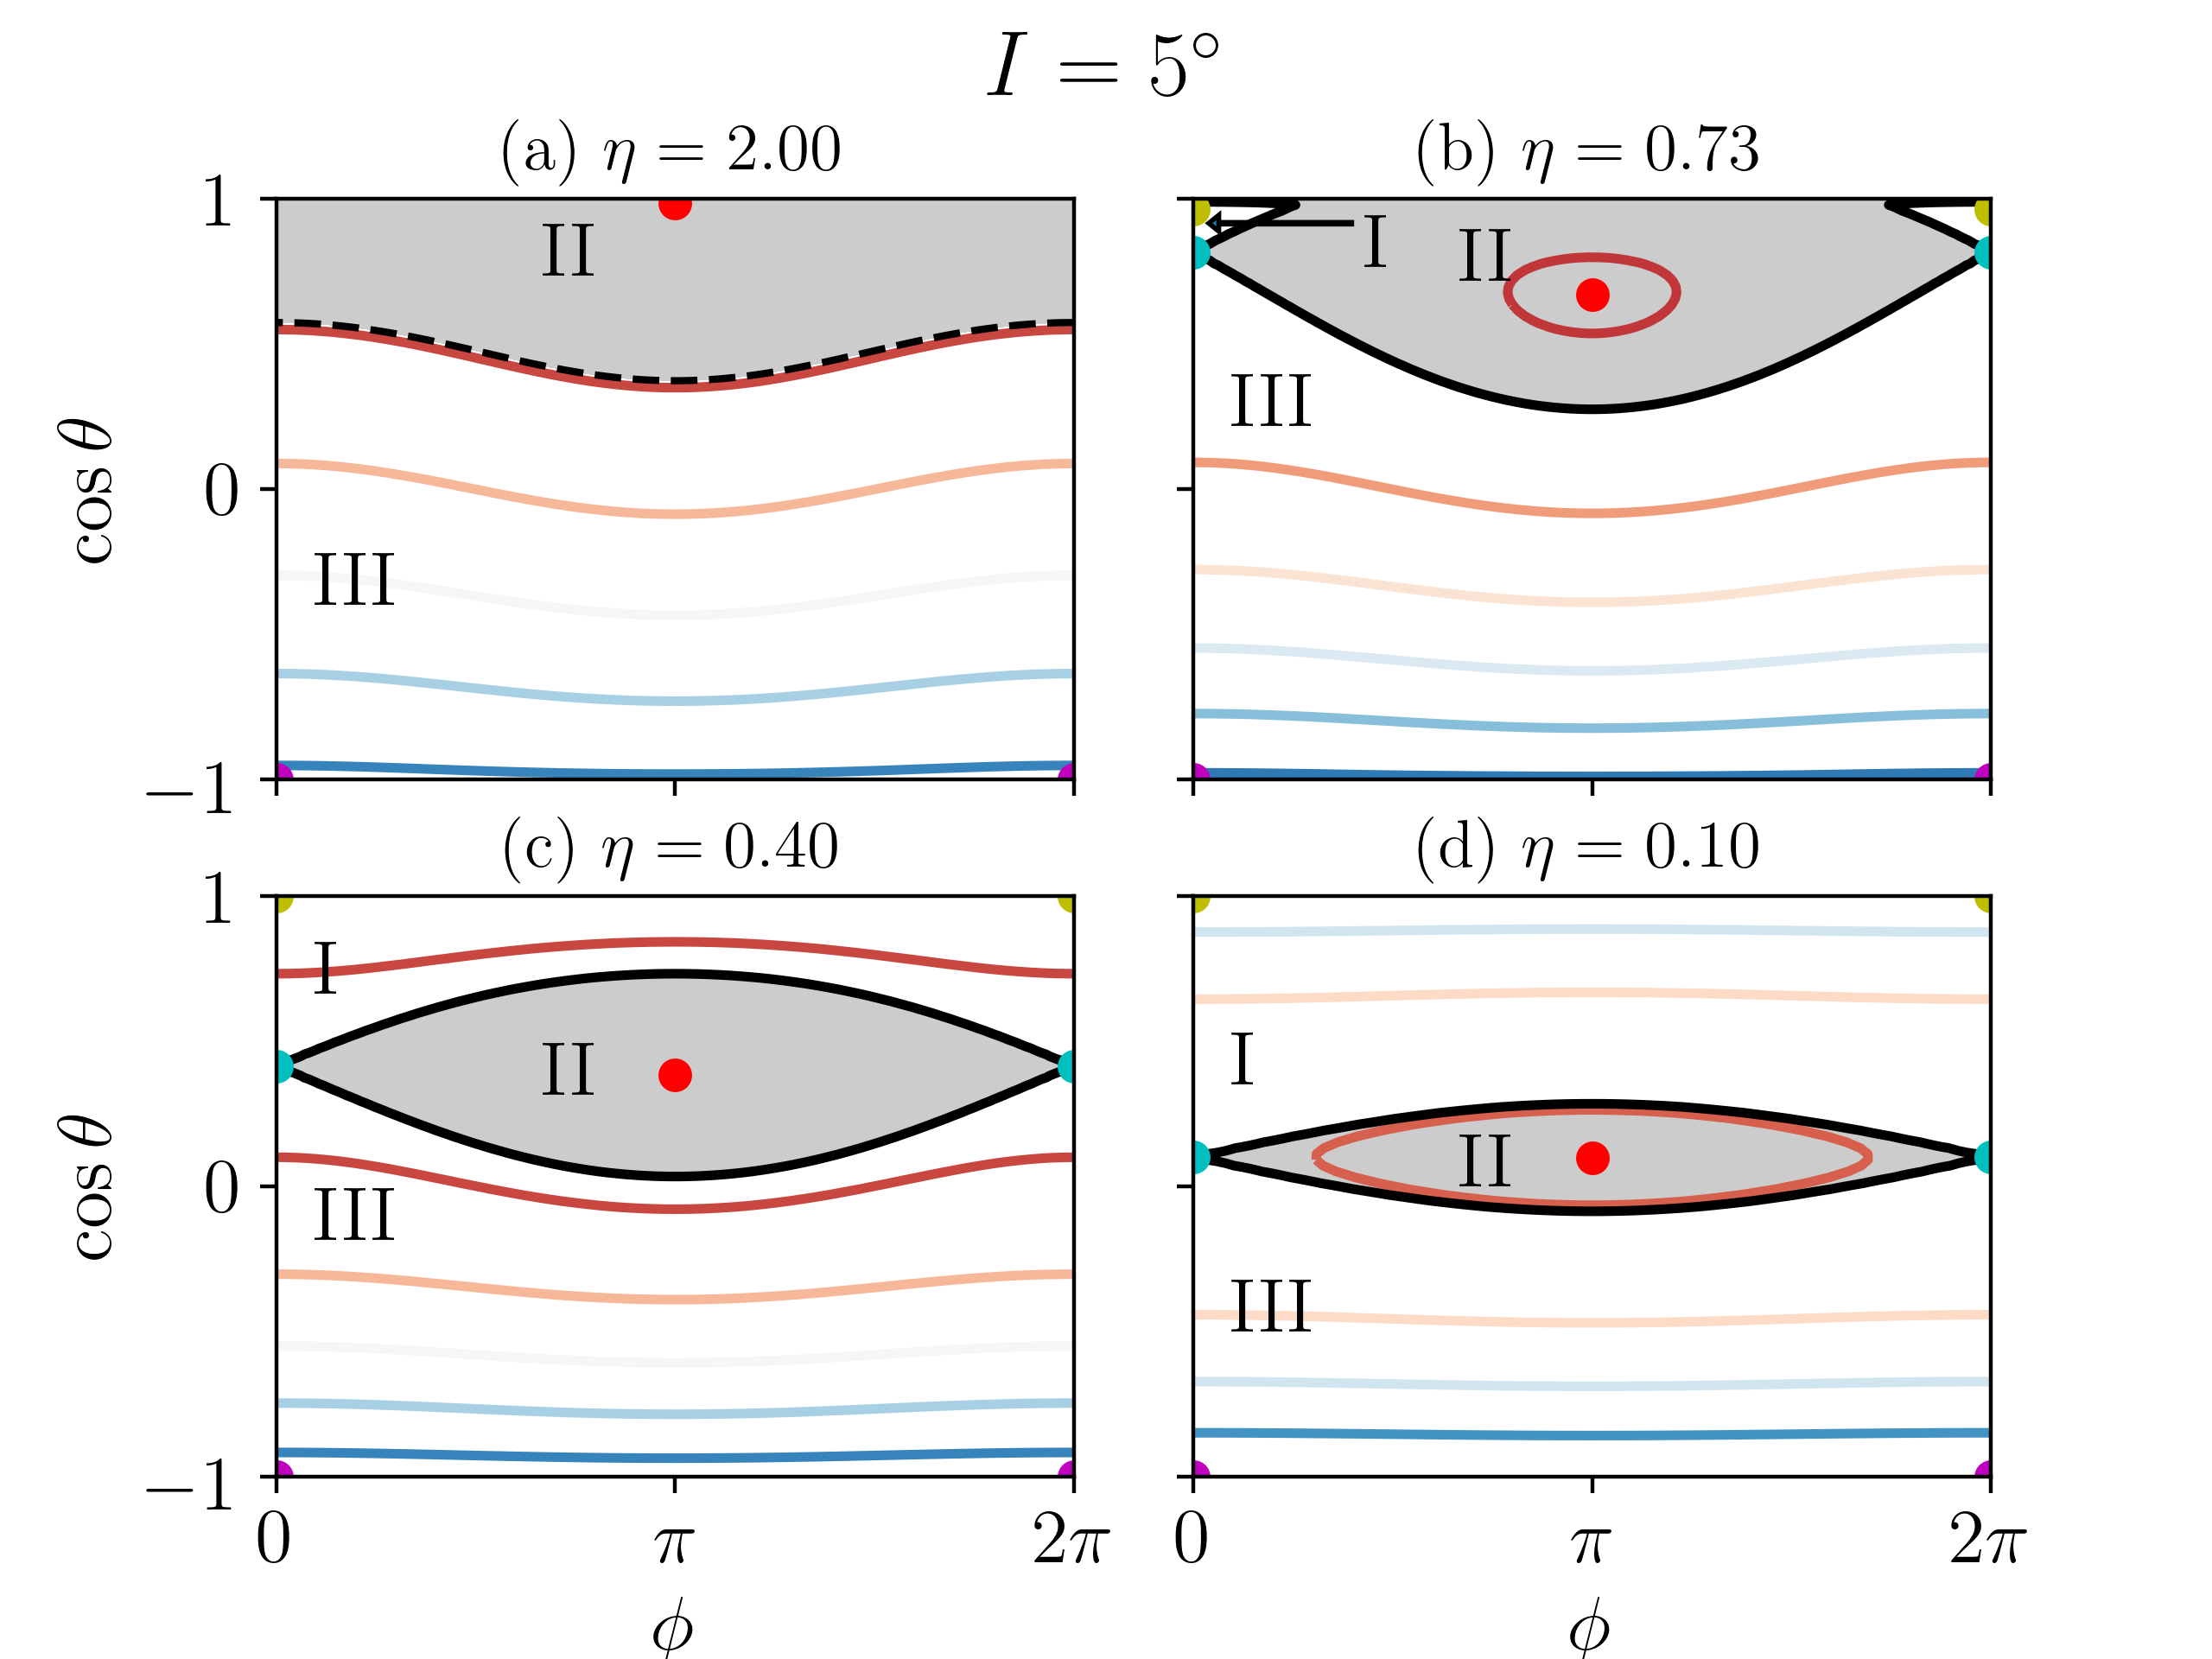
\includegraphics[width=\columnwidth]{../initial/0_eta/1contours_flip.png}
    \caption{Contour plot of $H\p{\phi, \cos \theta}$, where warmer colors
    denote more positive values. The black solid line is the separatrix, which
    only exists for $\eta < \eta_c$. The three zones, divided by the separatrix,
    are labeled. The interior of the separatrix, shaded in grey, is formally
    only defined for $\eta < \eta_c$, but we may identify the phase space
    trajectories that flow into zone II when evolved forward in time; this is
    the shaded region in the top left plot, bounded by the dotted black
    line.}\label{fig:eq_1contours}
\end{figure}

The locations of the $\cos\theta$ of the two/four CSs as a function of $\eta$ is
provided in \autoref{fig:cs_locs}.
\begin{figure}
    \centering
    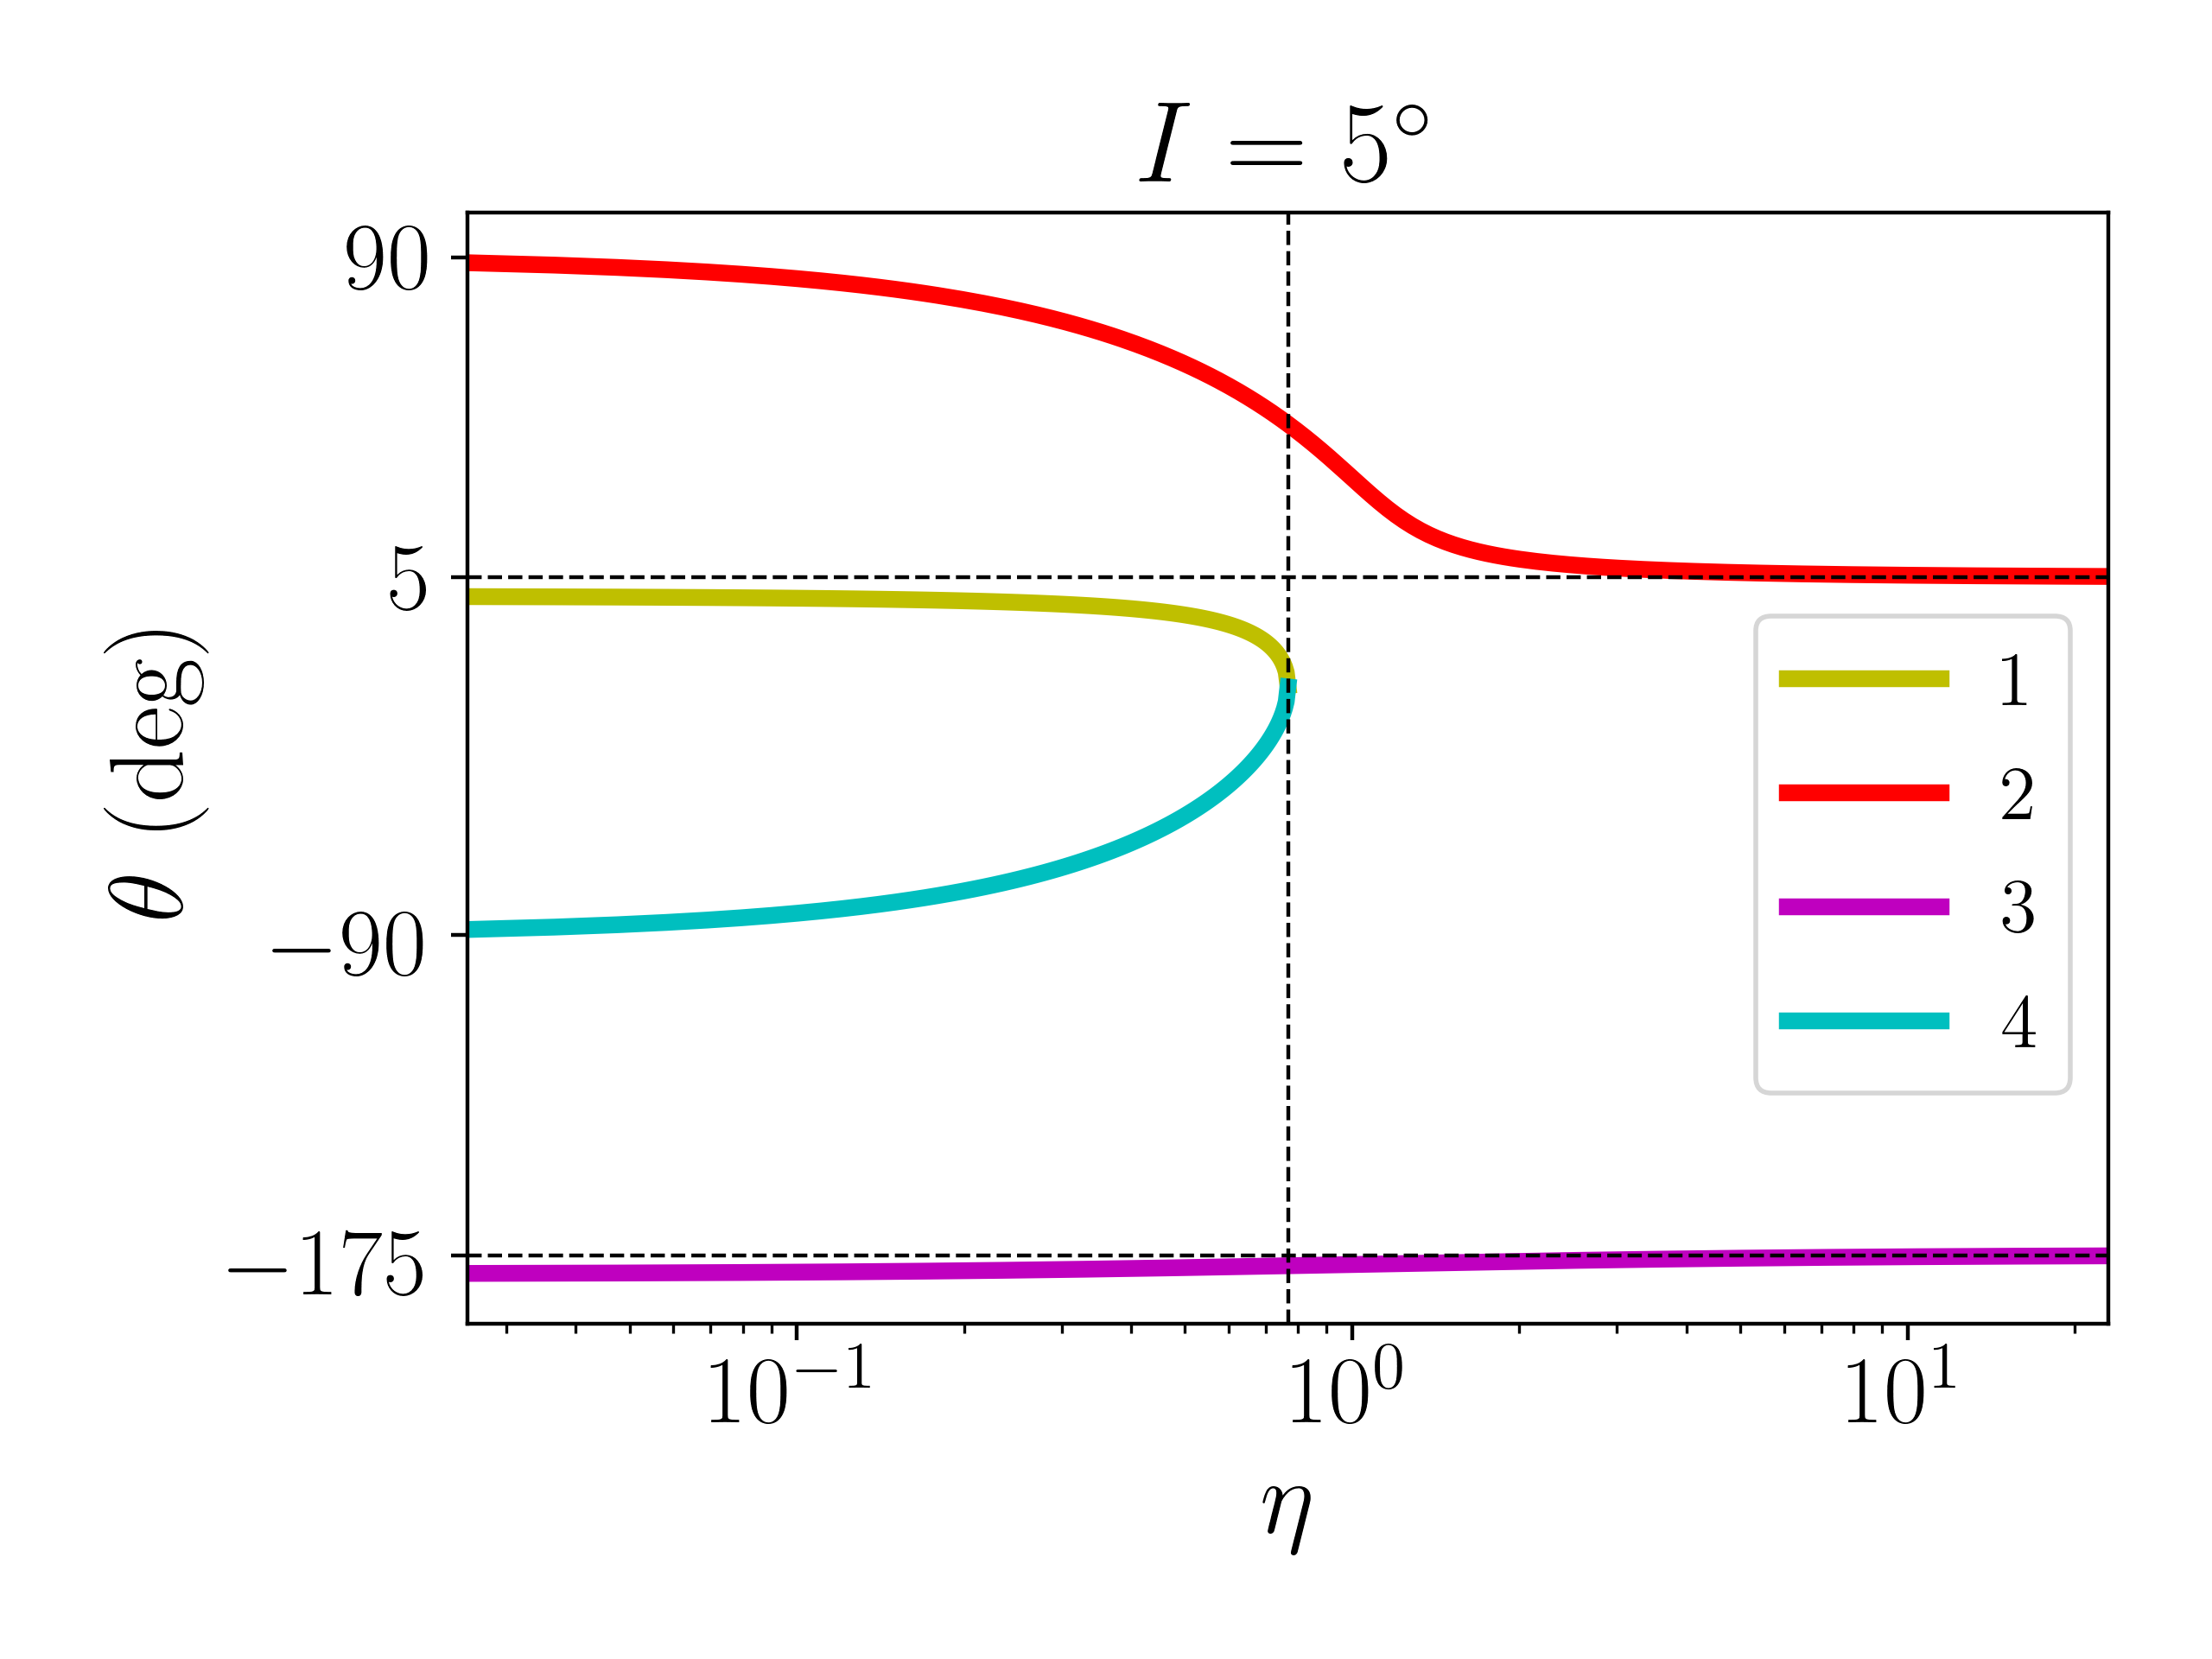
\includegraphics[width=\columnwidth]{../initial/99_misc/2_cs_locs.png}
    \caption{$\theta$ values of the Cassini states over time, following the same
    coloring scheme as \autoref{fig:eq_1contours}. Note that $\theta \in [-\pi,
    \pi]$ is the traditional definition of the polar angle
    \citep[see e.g.][]{colombo1966,peale1969,henrard1987}.}\label{fig:cs_locs}
\end{figure}

\subsection{Separatrix}

In the four-CS regime, one of the CSs is a saddle point, conventionally denoted
Cassini State 4 (CS4). All trajectories are periodic with finite period except
two critical trajectories asymptotic in the past and future to CS4. Together,
these two critical trajectories are referred to as the \emph{separatrix} and
divide phase space into three zones. We label these zones as illustrated in
\autoref{fig:eq_1contours}. As trajectories of constant $\eta$ evolve along
contours of constant $H$, it can be observed that trajectories in zone II
librate about CS2 while those in zones I/III circulate.

The unsigned areas of the three zones are known exactly in literature
\citep{henrard1987,ward2004I}. Defining
\begin{align*}
    z_0 &= \eta\cos I, &
    \chi &= \sqrt{-\frac{\tan^3\theta_4}{\tan I} - 1},\\
    \rho &= \chi \frac{\sin^2 \theta_4\cos \theta_4}{
        \chi^2 \cos^2\theta_4 + 1},&
    T &= 2\chi \frac{\cos \theta_4}{
        \chi^2 \cos^2\theta_4 - 1},\\
\end{align*}
the areas for $\eta < \eta_c$ are given by
\begin{subequations}\label{se:area_ward}
    \begin{align}
        A_{II} &= 8\rho + 4\arctan T - 8z_0 \arctan \frac{1}{\chi},\\
        A_I &= 2\pi\p{1 - z_0} - \frac{A_2}{2},\\
        A_{III} &= 2\pi\p{1 + z_0} - \frac{A_2}{2}.
    \end{align}
\end{subequations}
These are plotted as a function of $\eta$ in \autoref{fig:eq_areas}. Note that
the zones are not formally defined for $\eta > \eta_c$, but a natural extension
exists: evolve an initial point $p$ under adiabatic decrease of $\eta > \eta_c$
until the separatrix appears at $\eta = \eta_c$, then identify $p$ with the zone
it is in at $\eta_c$. Since phase space area is conserved under adiabatic
evolution, this implies $A_i\p{\eta > \eta_c} = A_i(\eta_c)$.
\begin{figure}
    \centering
    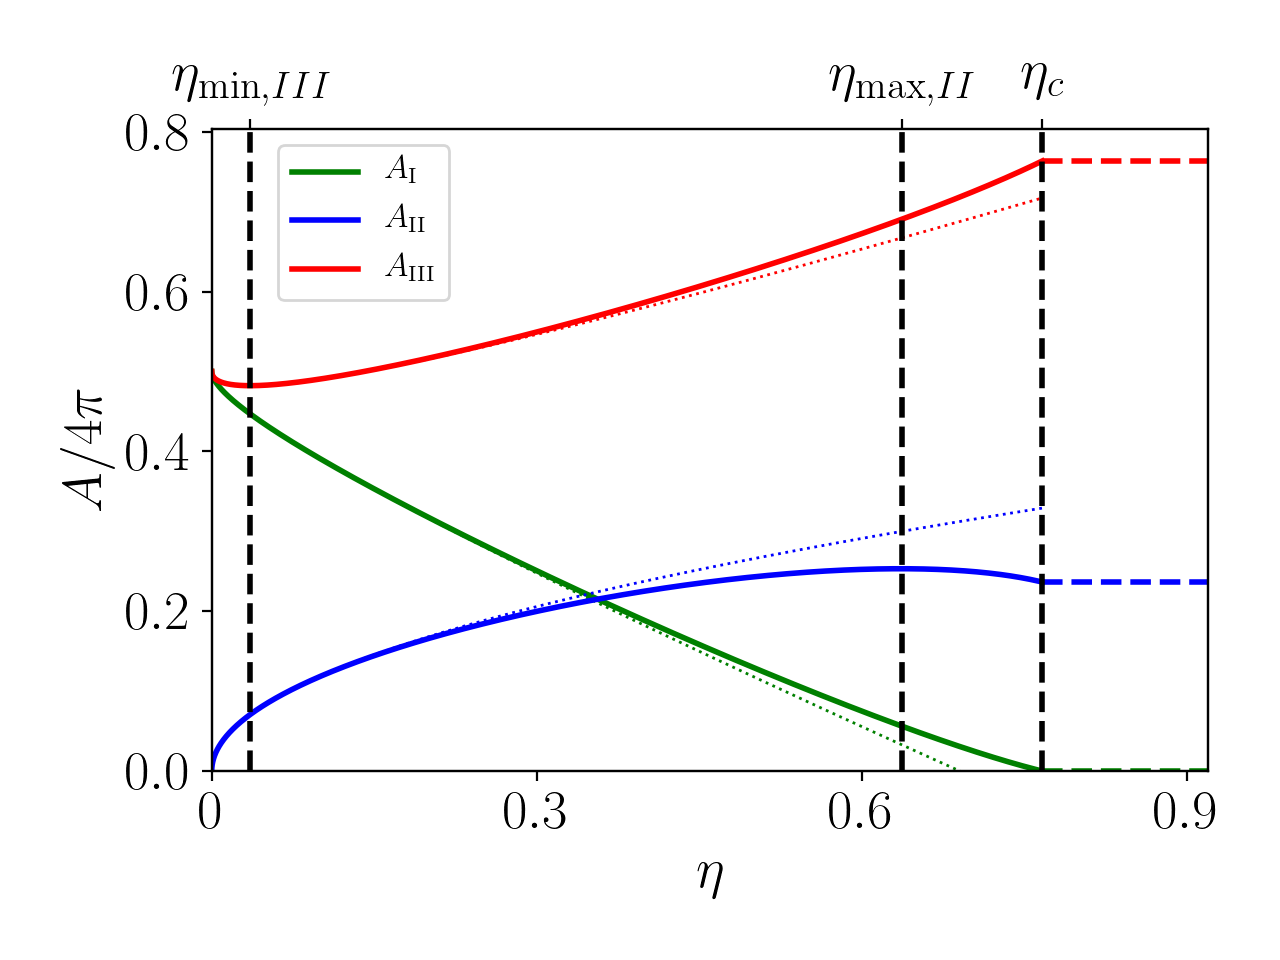
\includegraphics[width=\columnwidth]{../initial/99_misc/1_areas.png}
    \caption{Plot of fractional $A_{i}(\eta)$ as given by
    \autoref{se:area_ward}. Dotted lines correspond to small $\eta$
    approximations discussed in \autoref{ss:app_transition}. Dashed lines denote
    effective values of $A_{II}, A_{III}$ for $\eta > \eta_c$, denoting the
    area of points that would flow into either area under adiabatic decrease of
    $\eta$ to below $\eta_c$.}\label{fig:eq_areas}
\end{figure}

\section{Adiabatic Evolution}\label{s:ad}

As $\eta$ decreases, the trajectory generally encounters the separatrix at some
value $\eta_\star$ depending on its initial condition. If $\eta$ changes
sufficiently little during this separatrix-crossing orbit, the evolution of the
system is considered \emph{adiabatic}. In the truly adiabatic limit, $\epsilon
\to 0$; we use $\epsilon = 3 \times 10^{-4}$ unless otherwise noted.

One criterion for adiabaticity is that the separatrix crossing timescale be
longer than the the resonant libration period \citep{ward2004I}. This is
evaluated in~\cite{millholland_disk}, and in our problem reduces to
\begin{equation}
    \at{\rd{\eta}{t}}_{cross} = -\epsilon\eta_\star \gtrsim
        -\sin\theta \sin I \cos I.\label{eq:ad_constr}
\end{equation}
Note that this is a necessary but not sufficient criterion: the libration period
is longer for trajectories nearer the separatrix and diverges at the separatrix
for constant $\eta$.

\subsection{Fiducial Simulation: Zone Transition Histories}\label{ss:ad_fid}

In the limit $\eta \to 0$, zone II disappears and all trajectories circulate at
constant final $\theta$ values, notated $\theta_f$. We run simulations that
terminate at $\eta = 10^{-{-3.5}}$ and measure $\theta_{f}$. We vary the initial
value of $\theta_{sd}$, notated $\theta_{sd, i}$, among our simulations.

Initially, in the $\eta > \eta_c$ regime, only zones $II, III$ exist.
Conversely, at the end of the simulation when $\eta \to 0$, only zones $I, III$
exist. Naively then, one might expect four sequences of transitions
between zones (we call these dynamical ``tracks'') to appear during simulations:
(i) $II \to I$, (ii) $II \to III$, (iii) $III \to I$, and (iv) the trivial $III
\to III$ where the trajectory never encounters the separatrix. In fact, (v) a
fifth possible track involving two transitions is observed $III \to II \to I$.

Between zone transitions, the enclosed phase space area $A \equiv \oint \cos\theta
\;\mathrm{d}\phi$ is an adiabatic invariant. Here, we adopt convention $A$ is a
\emph{signed} area
\begin{equation}
    A = \oint \p{1 - \cos \theta}\;\mathrm{d}\phi.
\end{equation}
This has the advantage of (i) having a removable singularity when the trajectory
crosses $\cos \theta = 1$, and (ii) being easily expressible as combinations of
the $A_i$ of \autoref{se:area_ward}. The bounds of the integral are either a
libration or circulation cycle.

Given this definition, the change in $A$ during a separatrix encounter is easily
understood \citep{henrard1982}. We present in \autoref{fig:ad_21} a fiducial
simulation undergoing the $II \to I$ zone transition. An initial condition in
zone II with initial adiabatic invariant $A_i > 0$ librates about CS2 until
$A_{II} = A_i$. At this point, it encounters the separatrix and moves into zone
I and the final enclosed phase space area is $A_f = -(A_{II} + A_{III})$.
Further simulations illustrating the other tracks are depicted in
\autoref{ss:app_tracks}.
\begin{figure}
    \centering
    \begin{subfigure}{\columnwidth}
        \centering
        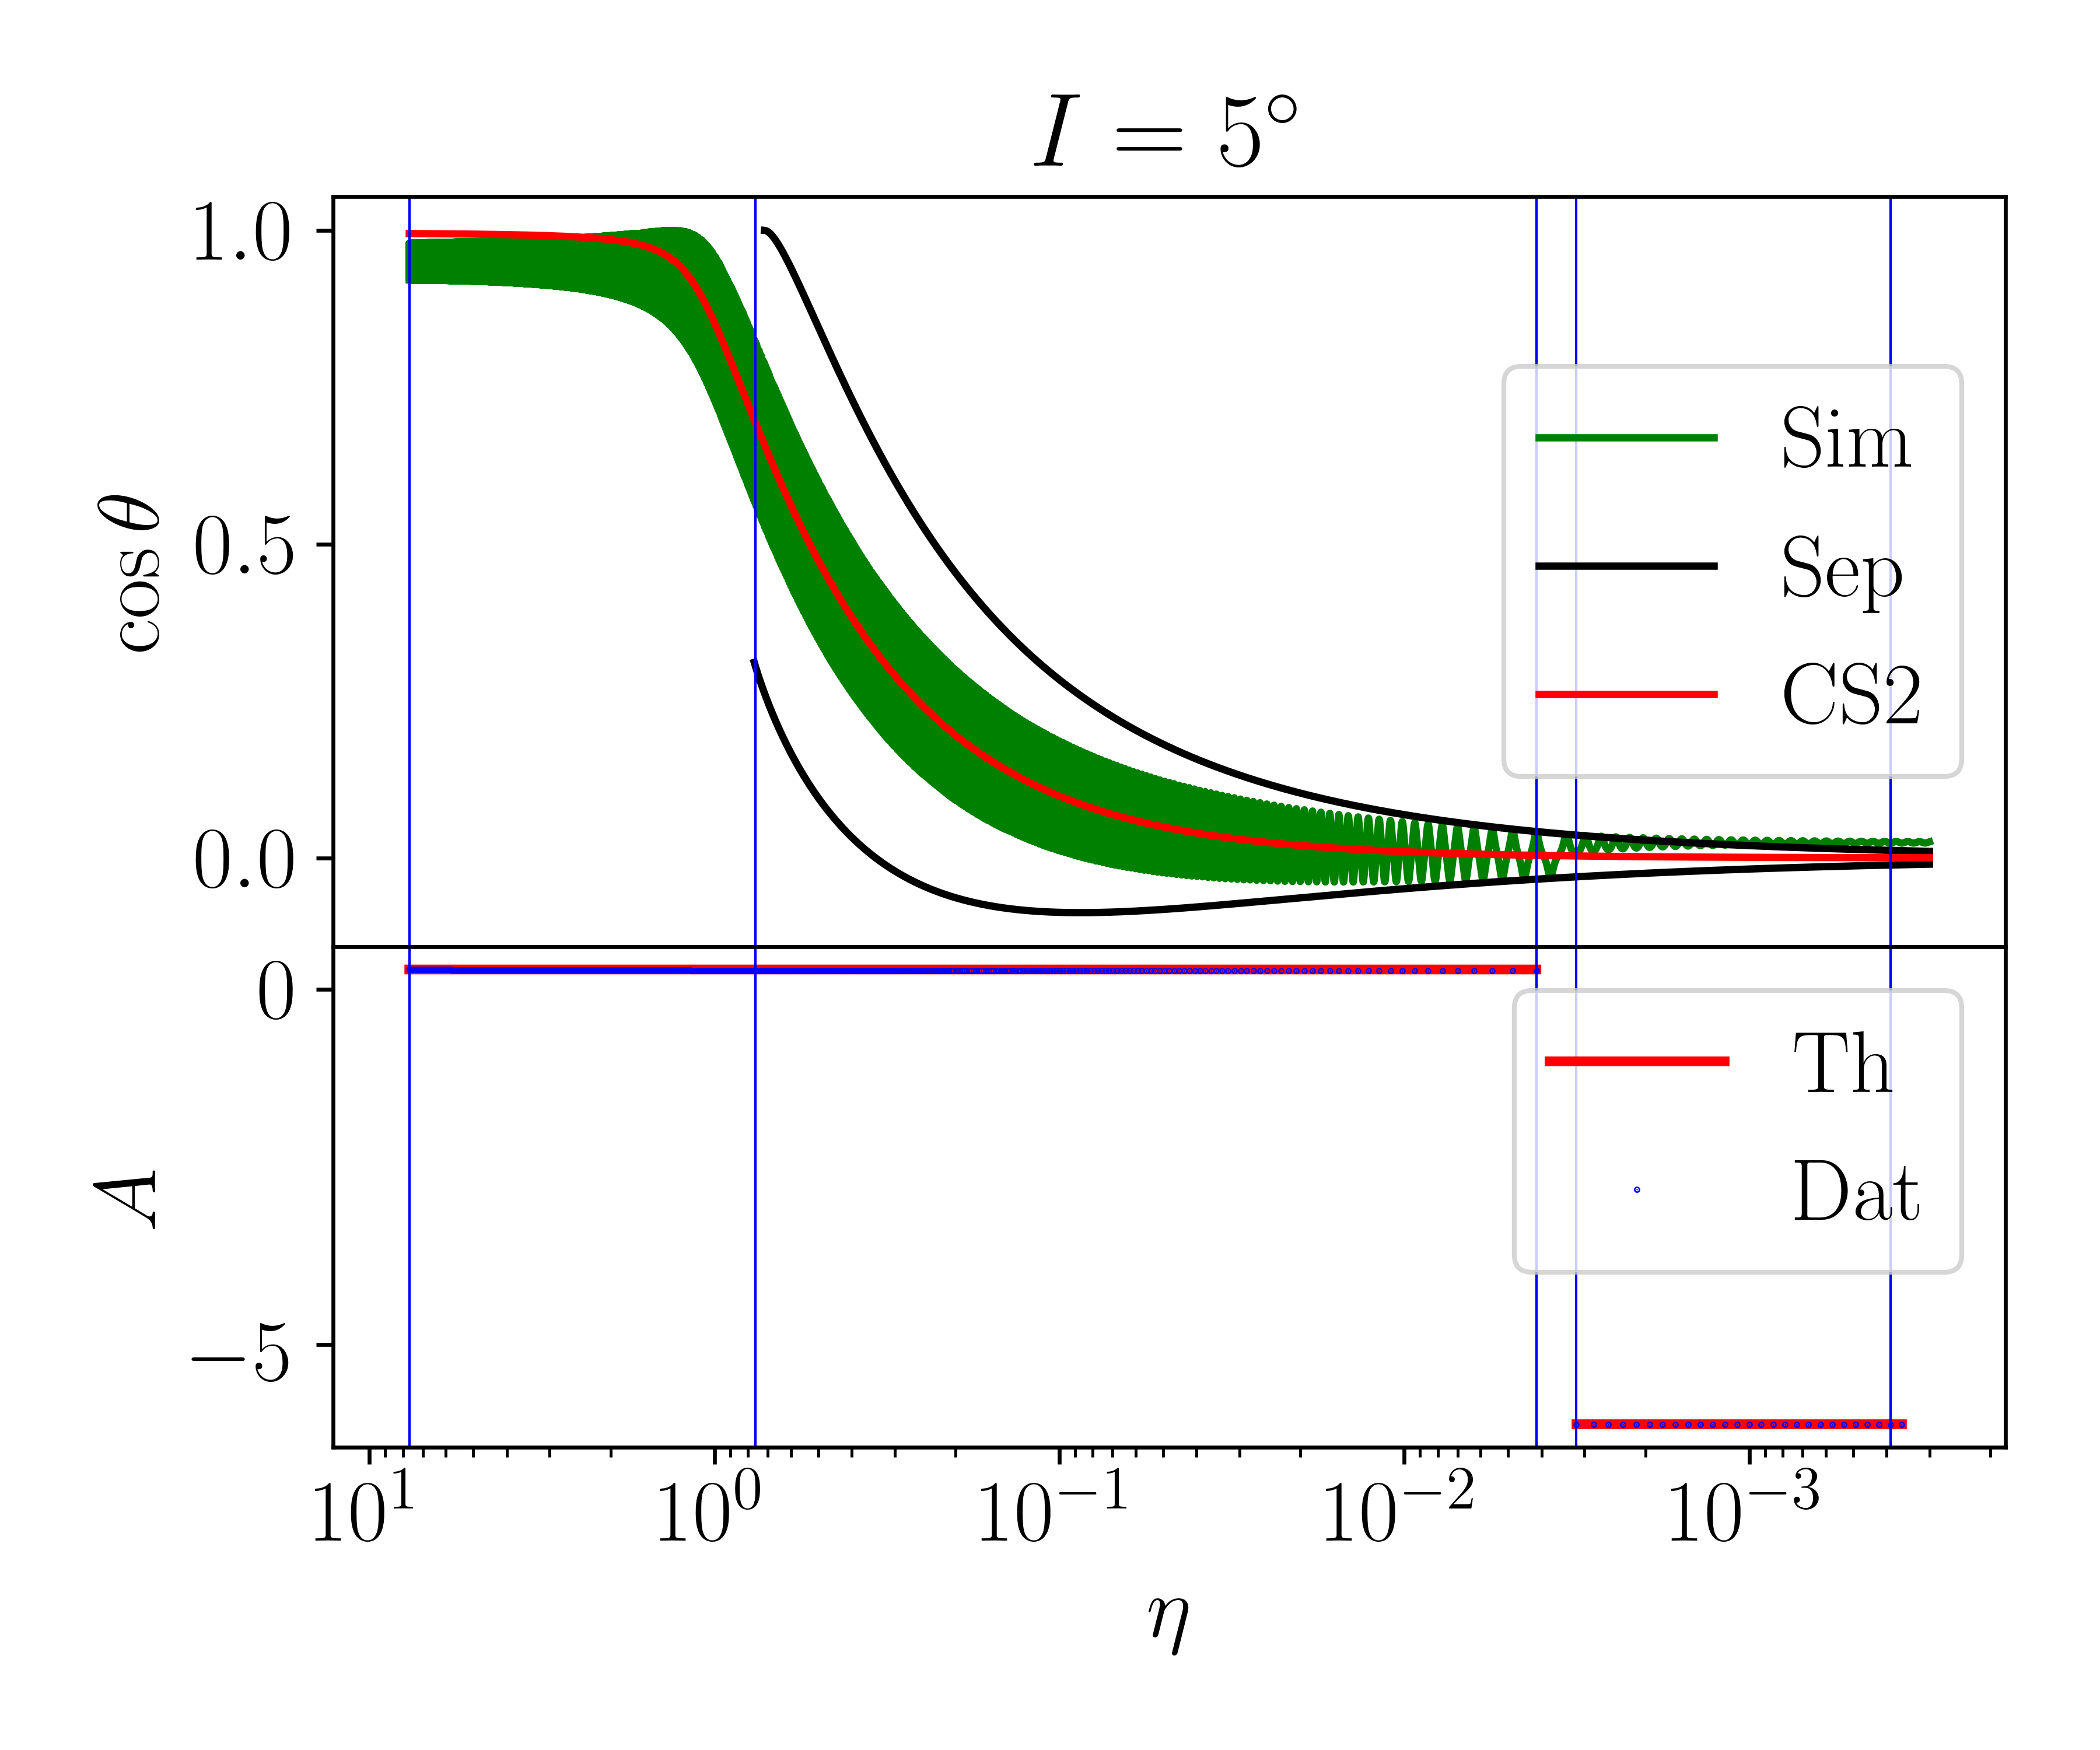
\includegraphics[width=\columnwidth]{../initial/2_toy2/3testo21.png}
    \end{subfigure}
    \begin{subfigure}{\columnwidth}
        \centering
        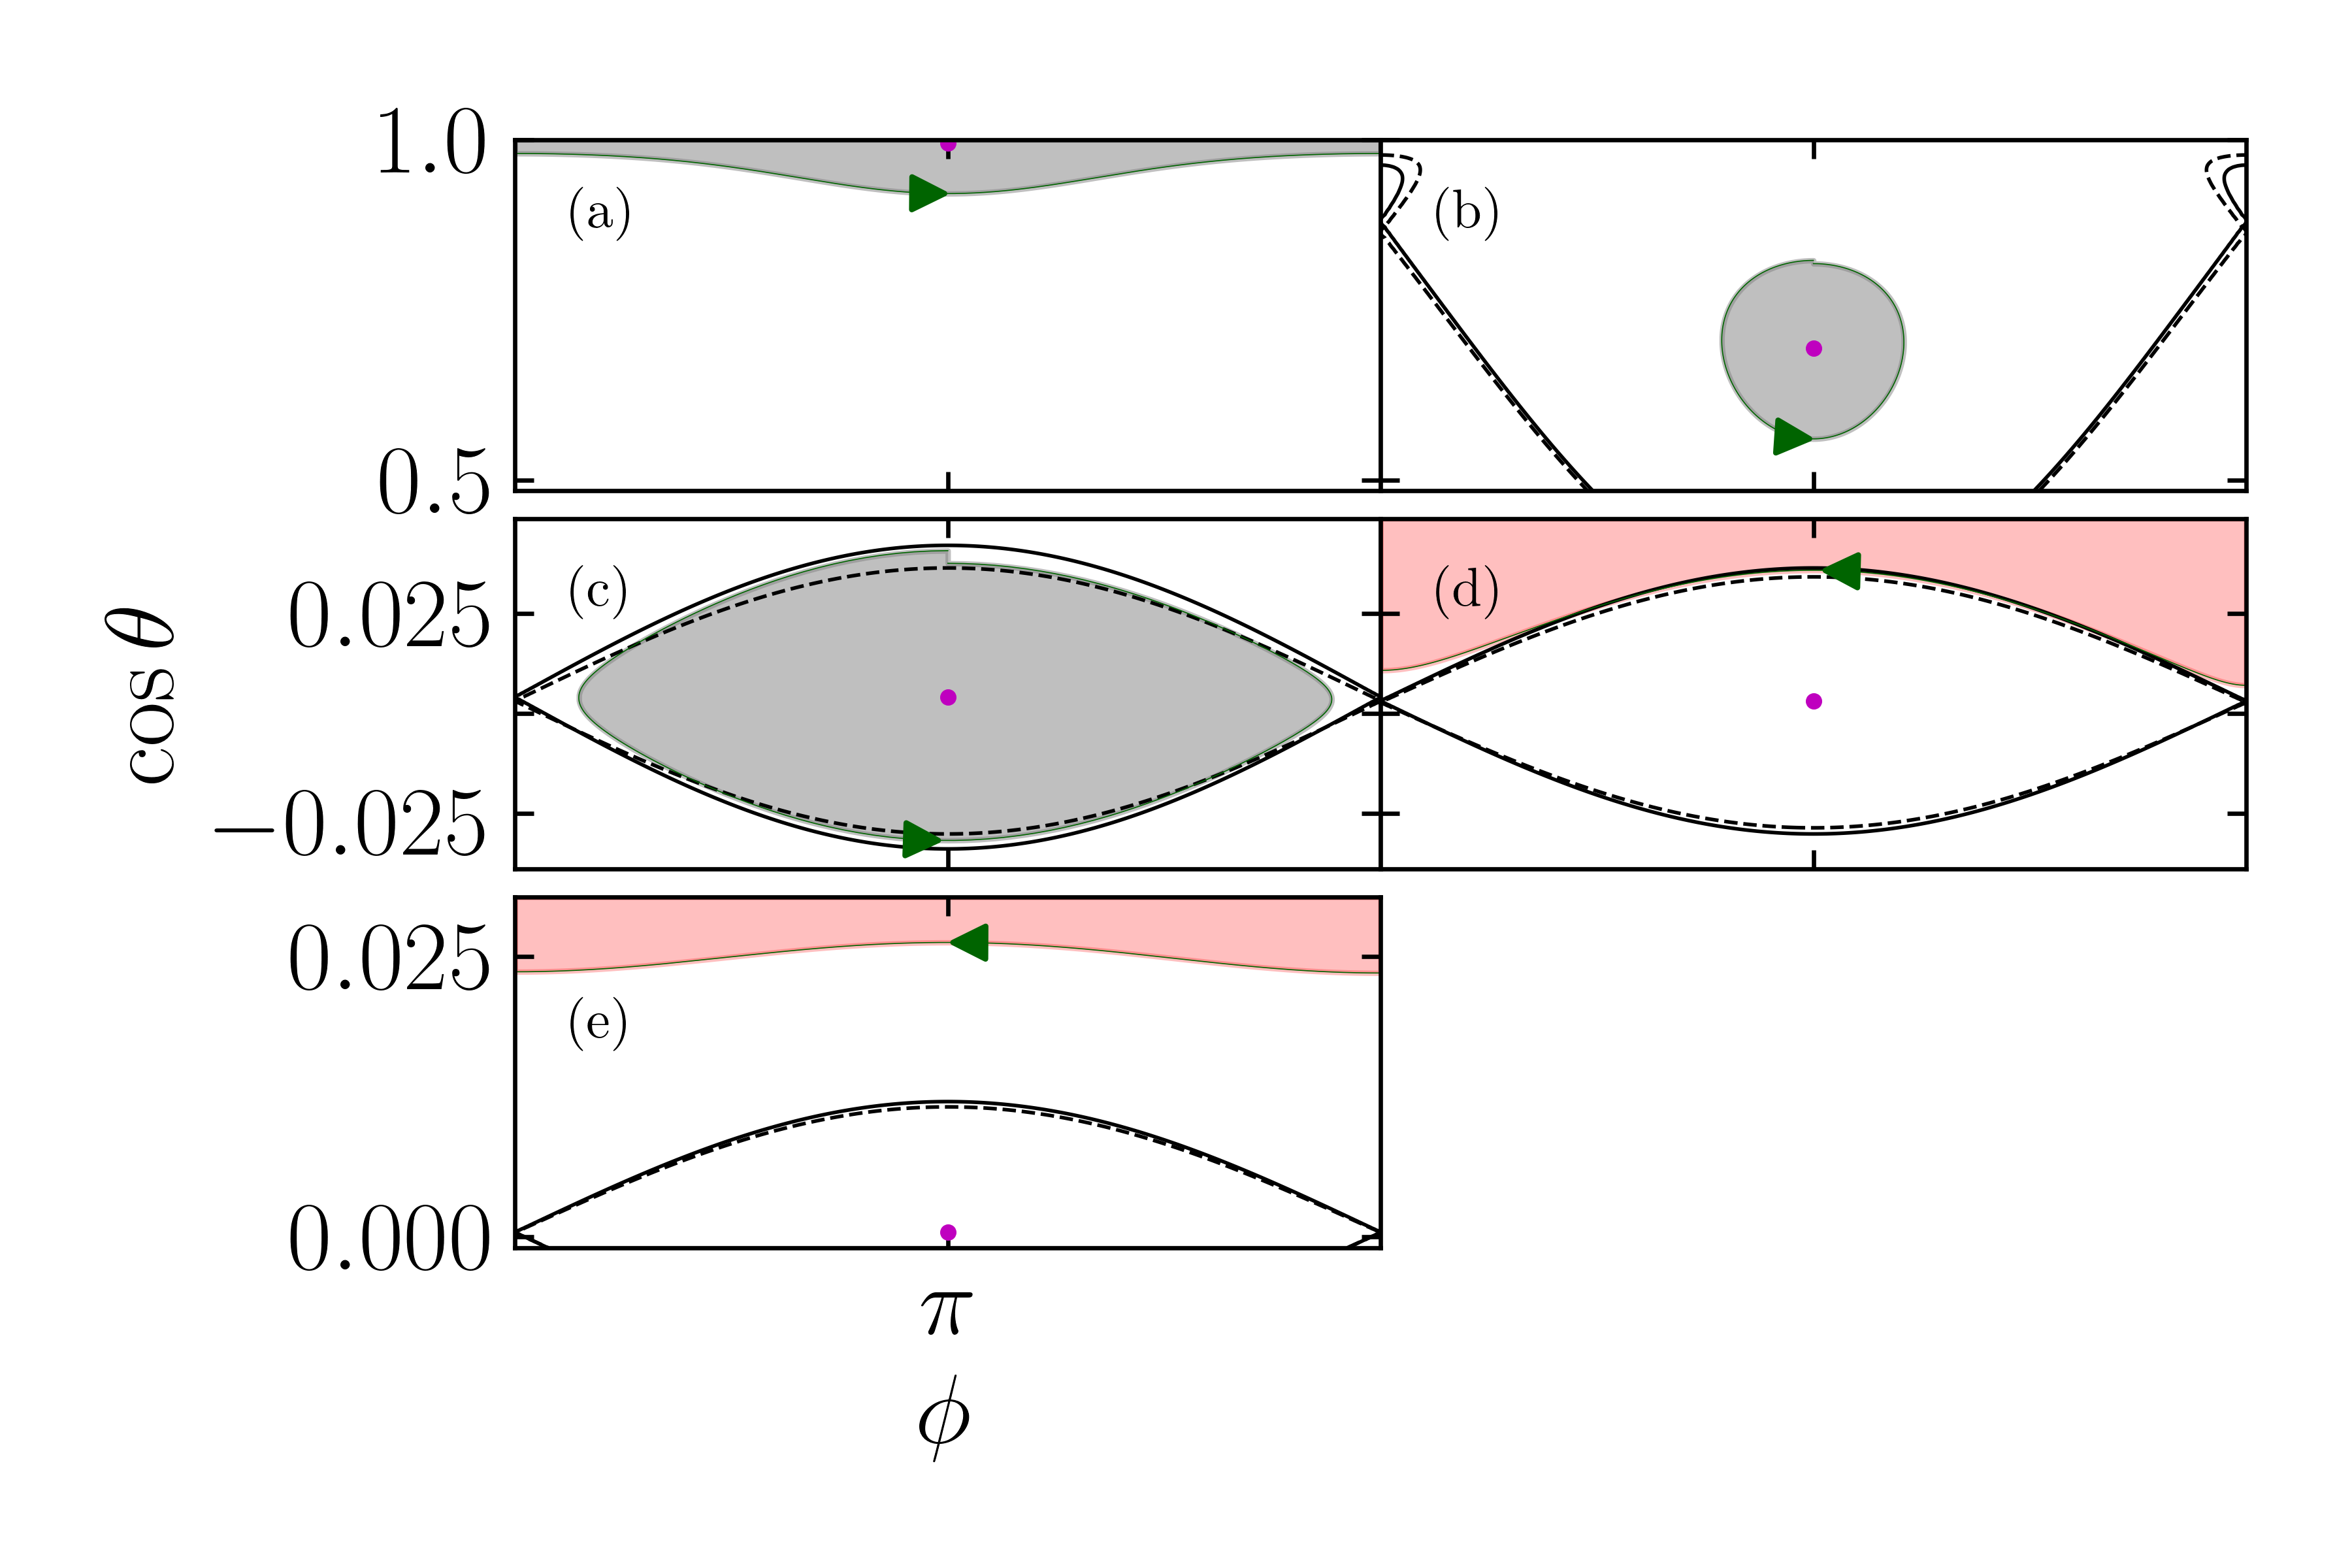
\includegraphics[width=\columnwidth]{../initial/2_toy2/3testo21_subplots.png}
    \end{subfigure}
    \caption{Fiducial simulation following the $A_{II} \to A_{I}$ transition. Top
    plot upper panel: plot of $\cos \theta(t)$ (gold) in an example simulation.
    Overlaid are the locations of Cassini State 2 (magenta), and upper and lower
    bounds on the separatrix (dashed black). Note that the trajectory
    successfully tracks CS2 to a misalignment angle $\theta \approx 90^\circ$.
    Vertical green lines denote times portrayed in bottom plot. Top plot lower
    panel: plot of the enclosed separatrix area obtained by integrating the
    simulated trajectory (blue dots) and adiabatic theory (red line). Lower
    plot: snapshots in the $\p{\cos \theta, \phi}$ space of the simulation
    trajectories for the times demarcated in green above, corresponding to the
    start of the simulation, the appearance of the separatrix, two panels
    depicting the separatrix crossing process, and a final snapshot at $\eta =
    10^{-3.5}$. Gold dots denote a full circulation or libration cycle at the
    selected time, while the separatrix at the start/end of the portrayed cycle
    are shown in solid/dashed black lines respectively. Also labeled is CS2
    (magenta).}\label{fig:ad_21}
\end{figure}

\subsection{Dynamical Outcomes}\label{ss:ad_ensemble}

In the adiabatic limit, while separatrix encounters induce discontinuous changes
in enclosed phase space, the outcomes of these encounters are well understood in
pioneering work by Henrard \citep{henrard1982,henrard1987}. For a wide range of
$\theta_{sd, i}$, we run simulations over a ring of initial conditions at each
$\theta_{sd, i}$ and measure the final $\theta_{ f}$ values. We can also
predict the values of $\theta_{ f}$ for each of the tracks as
well as their associated probabilities; refer to \autoref{ss:app_transition} for
details. The comparison of the final obliquities associated with these tracks
and those obtained via simulation can be seen in \autoref{fig:ad_ensemble}. The
same plot for $I = 10^\circ, I = 20^\circ$ can be found in
\autoref{ss:varying_I}.
\begin{figure}
    \centering
    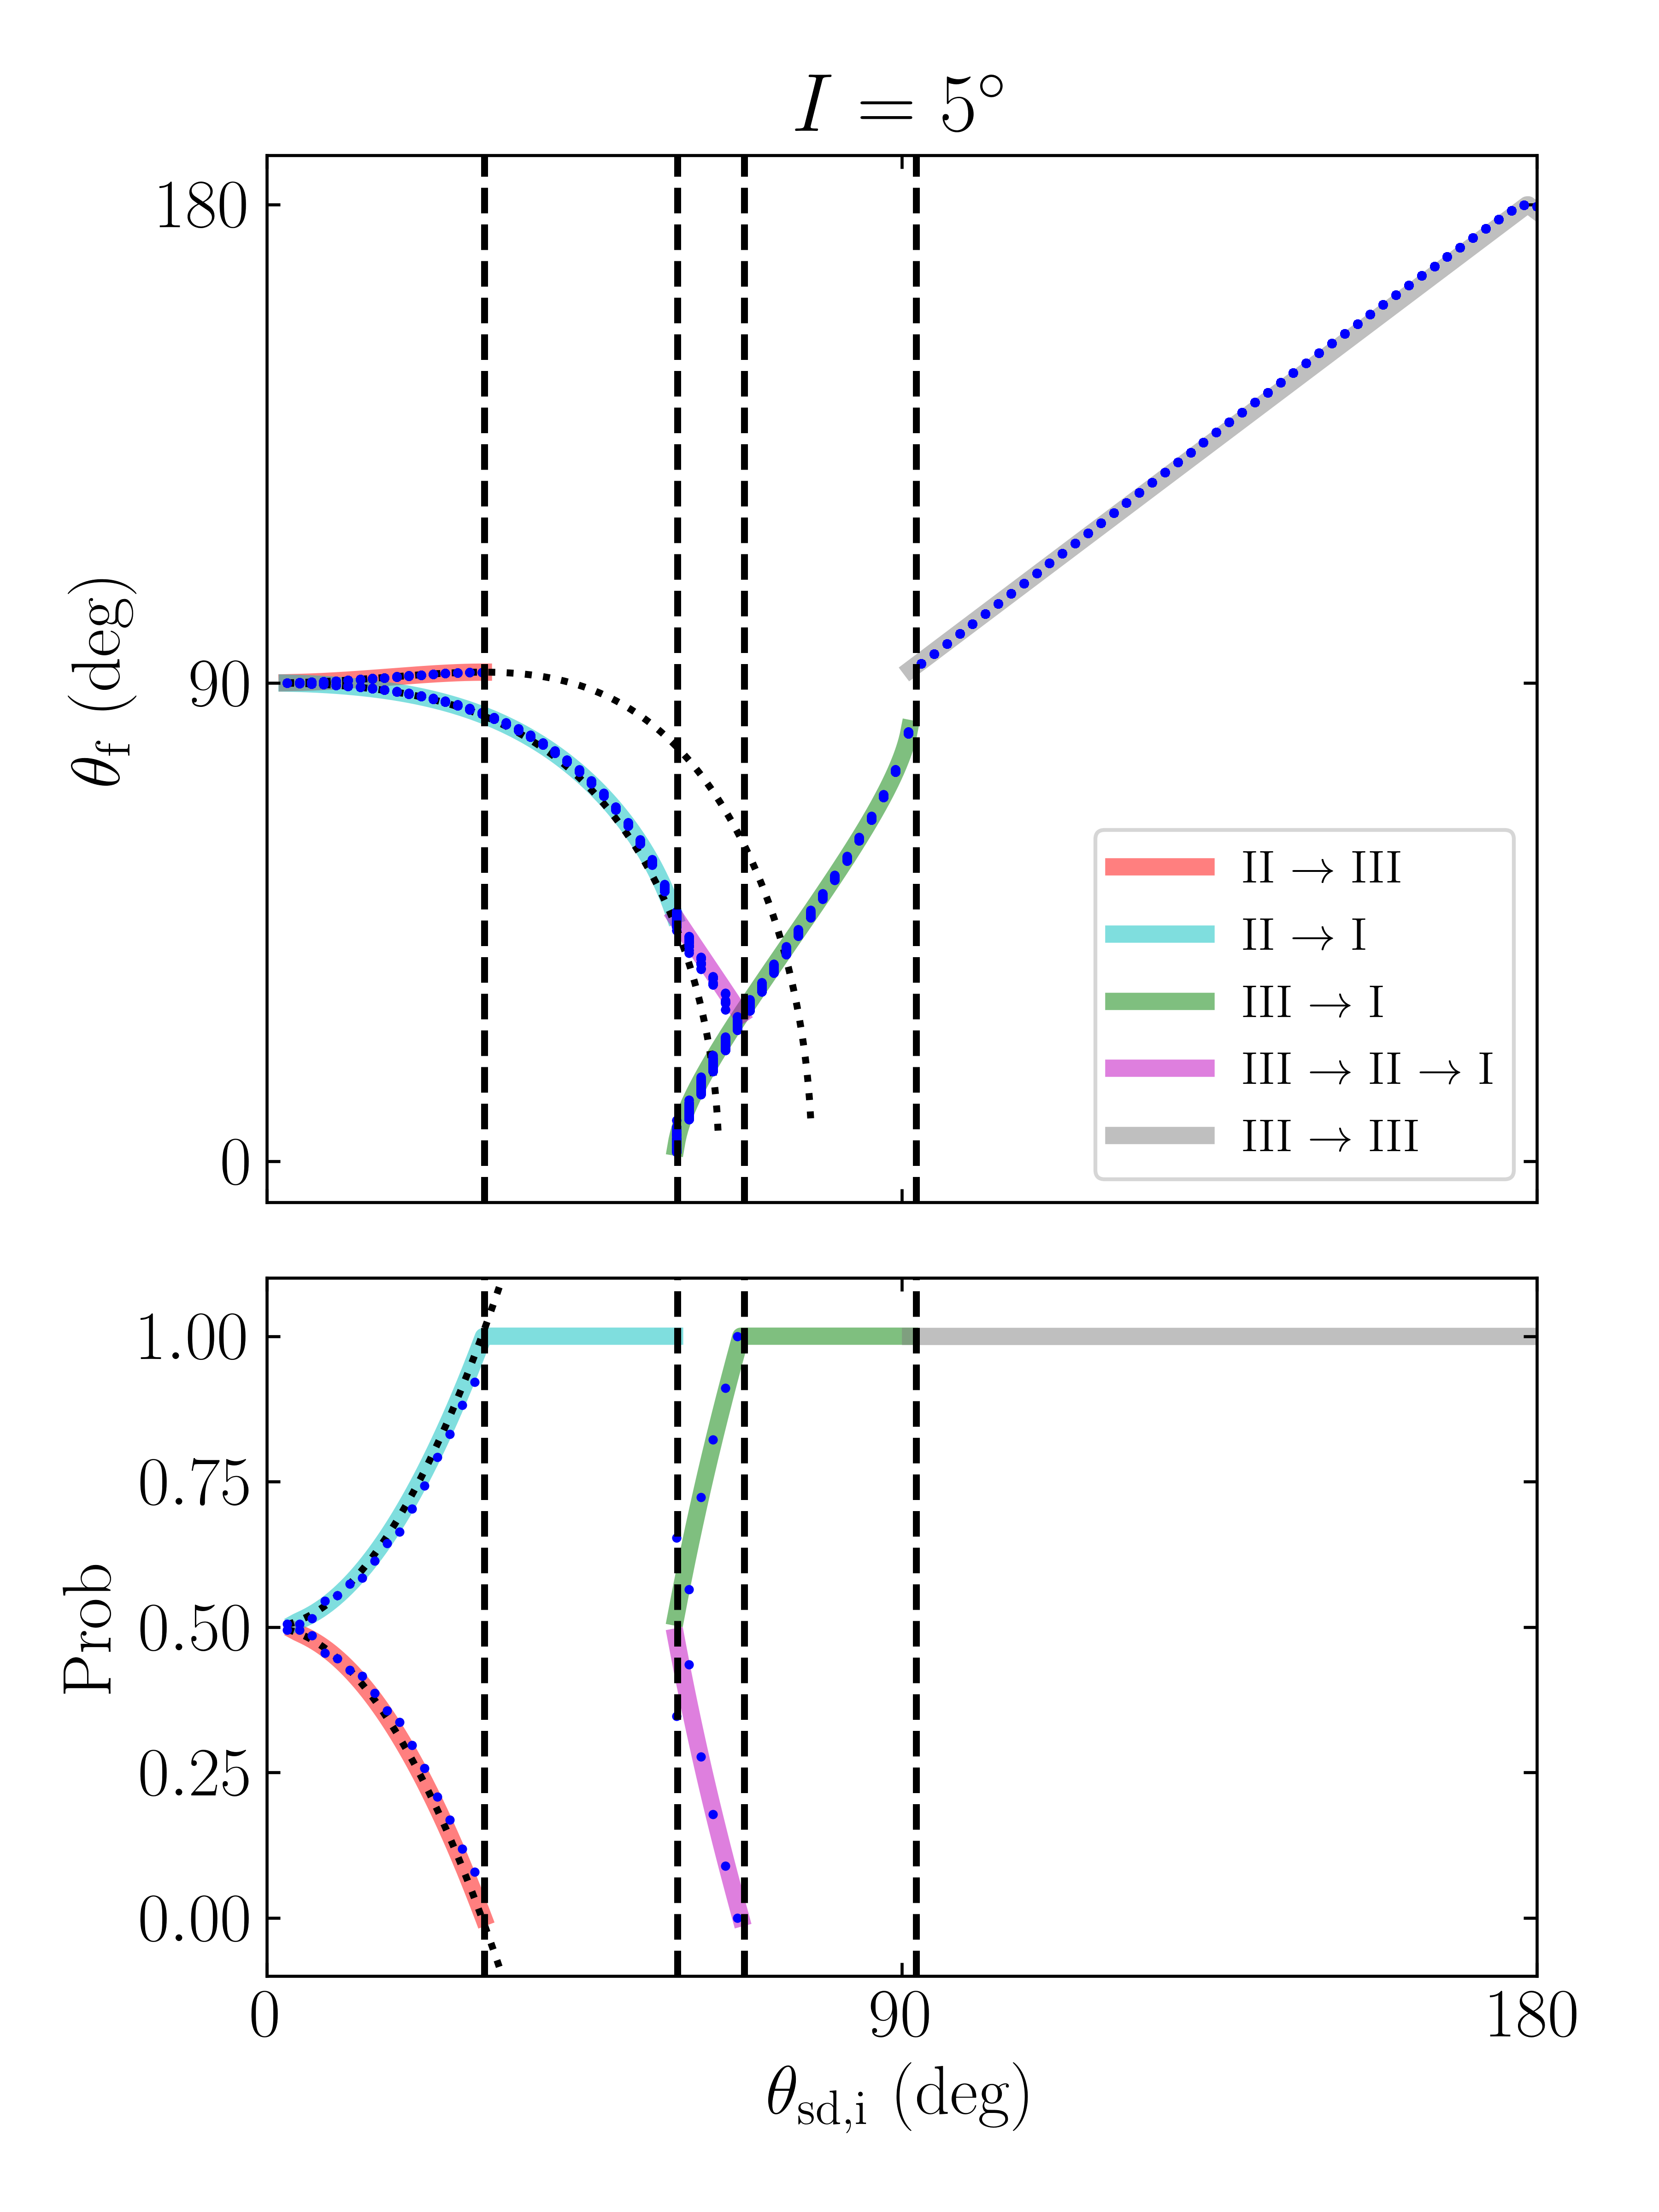
\includegraphics[width=\columnwidth]{../initial/2_toy2/3_ensemble_05_35.png}
    \caption{Top: $\theta_{f}\p{\theta_{sd, i}}$, overlaid with semi-analytic
    predictions of the $\theta_{ f}$ for each of the four nontrivial
    dynamical tracks in colored lines. Bottom: Semi-analytic probabilities of
    each of the dynamical tracks for each $\theta_{sd,
    i}$.}\label{fig:ad_ensemble}
\end{figure}

\subsection{Transition to Non-adiabaticity}

To illustrate the transition to non-adiabaticity, we present three simulations
with increasingly larger values of $\epsilon$ than \autoref{fig:ad_ensemble}
below in \autoref{fig:transition_to_nonad}.

At first non-adiabaticity manifests as a larger scatter of final obliquities
near the tracks predicted from adiabatic evolution. These scatters first set in
for trajectories starting in zone III, as these cross the separatrix at higher
values of $\theta$ and have a stricter adiabaticity criterion (see
\autoref{eq:ad_constr}).

Later, these large scatters take on band-like structures that seem to persist
across values of $\theta_{sd, i}$; we attribute these to the separatrix crossing
process becoming sensitive to the \emph{phase} of the final
libration/circulation orbit at separatrix crossing. This is equivalent to
separatrix crossing no longer being significantly slower than orbit timescales
and violating the adiabatic assumption.
\begin{figure}
    \centering
    \begin{subfigure}{\columnwidth}
        \centering
        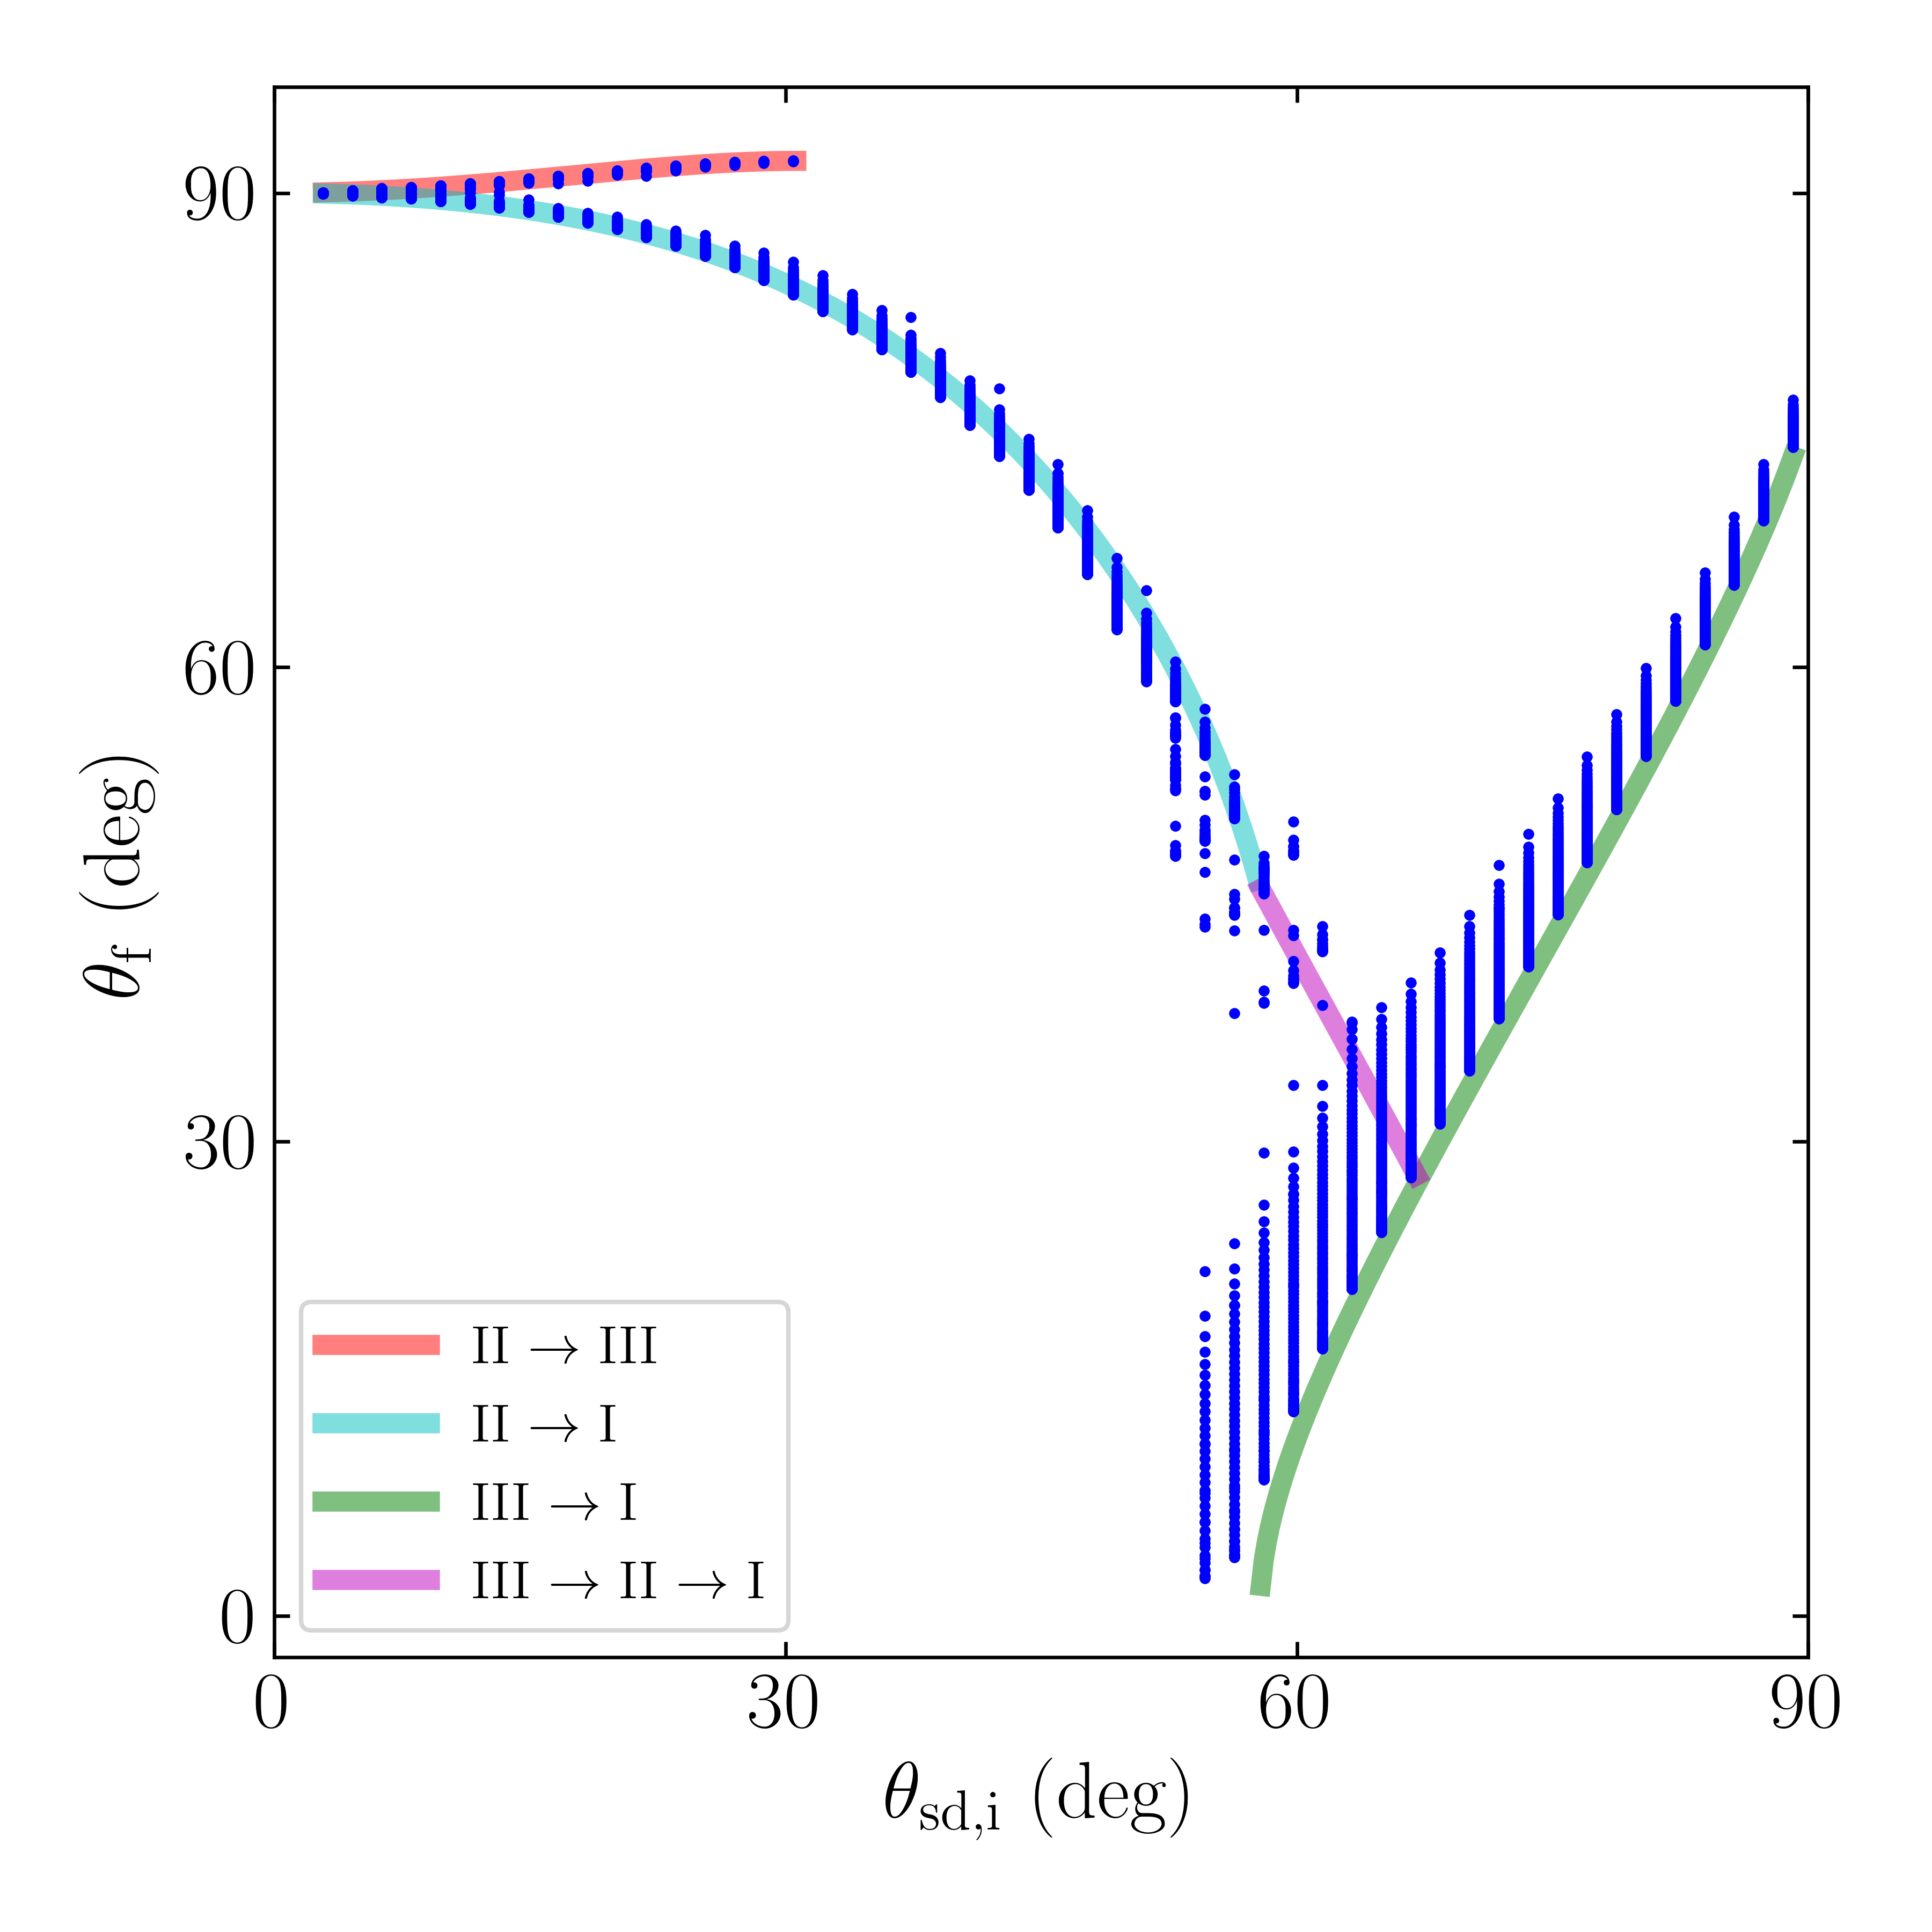
\includegraphics[width=\columnwidth]{../initial/2_toy2/3_ensemble_05_25.png}
    \end{subfigure}
    \begin{subfigure}{\columnwidth}
        \centering
        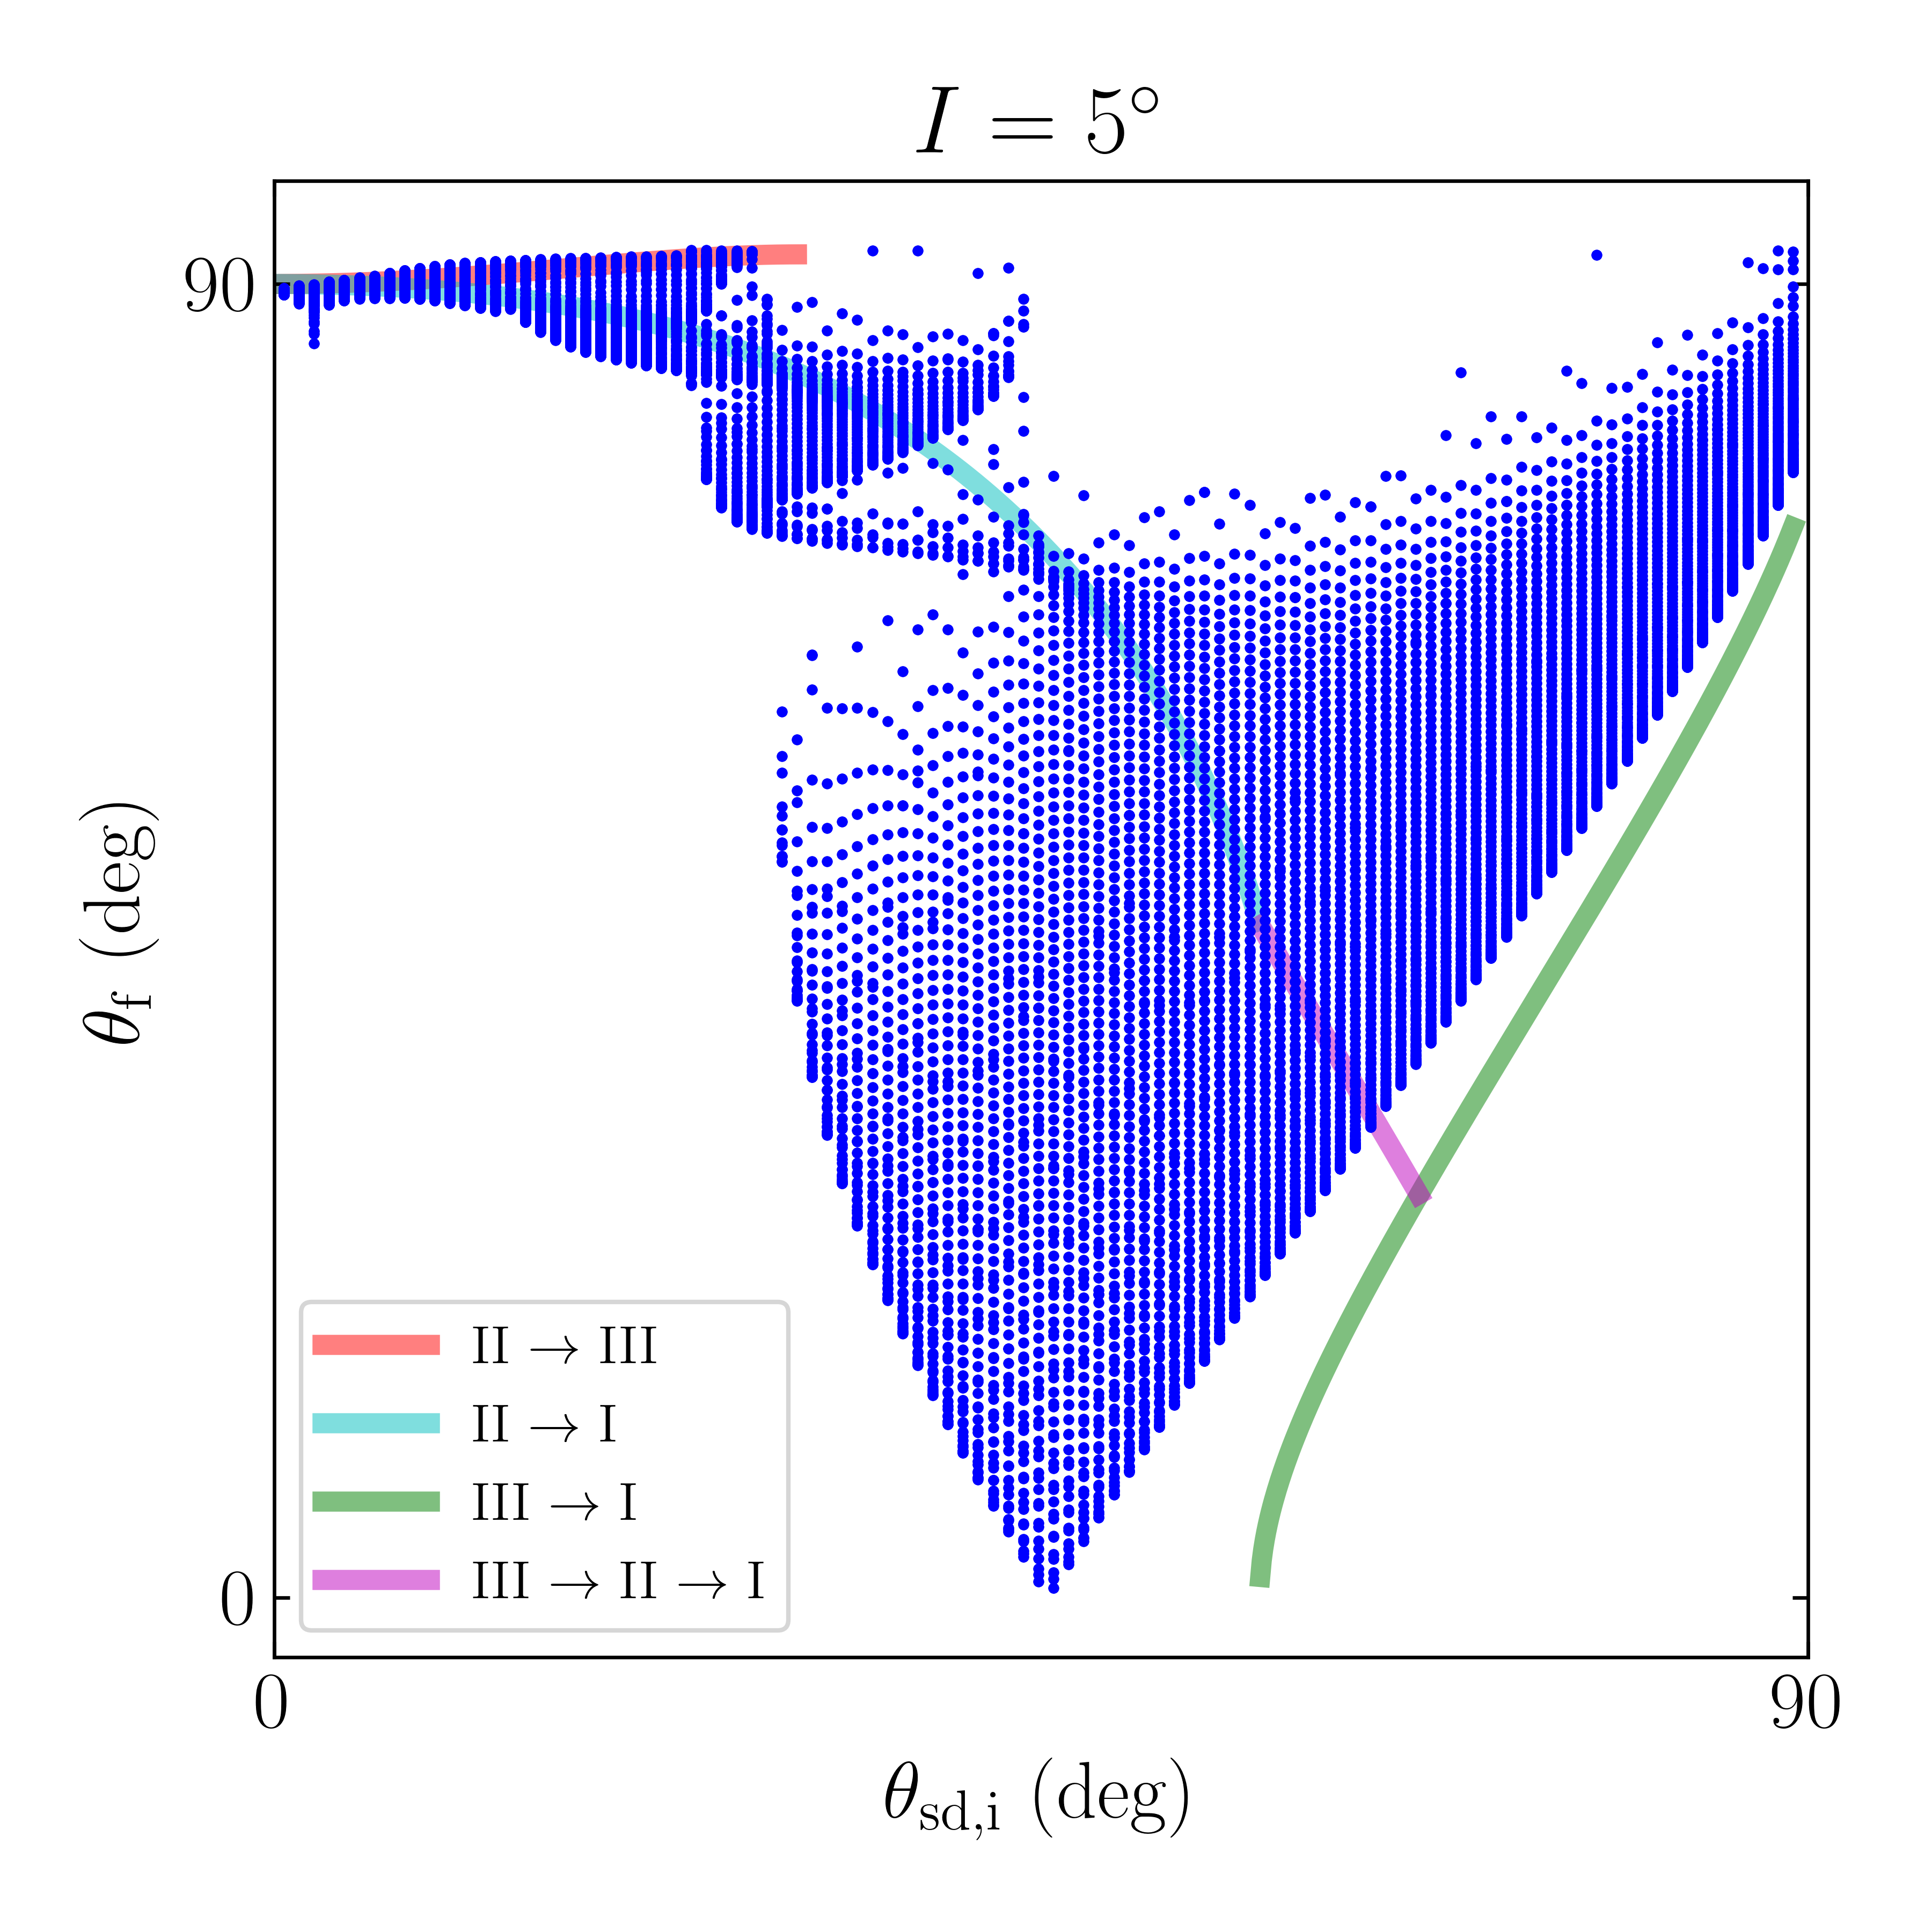
\includegraphics[width=\columnwidth]{../initial/2_toy2/3_ensemble_05_15.png}
    \end{subfigure}
    \begin{subfigure}{\columnwidth}
        \centering
        \includegraphics[width=\columnwidth]{../initial/2_toy2/3_ensemble_05_10.png}
    \end{subfigure}
    \caption{Increasingly larger $\epsilon$ used compared to those in
    \autoref{fig:ad_ensemble}. The general evolutionary tracks in the adiabatic
    limit deteriorate as $\epsilon$ is increased. Deviations from the adiabatic
    predictions seem to be banded structures, which can be attributed to
    non-adiabaticity ``freezing-in'' the phase of the obliquity variations over
    the final libration/circulation orbit prior to separatrix
    crossing.}\label{fig:transition_to_nonad}
\end{figure}

\section{Nonadiabatic Evolution}\label{s:nonad}

Here, we consider $\epsilon \sim 0.2$ which significantly violates
\autoref{eq:ad_constr}.

\subsection{Sample Trajectory}

A sample trajectory following in the style of \autoref{fig:ad_21} but for
$\epsilon = 0.1$ is provided in \autoref{fig:nonad_traj}.
\begin{figure}
    \centering
    \begin{subfigure}{\columnwidth}
        \centering
        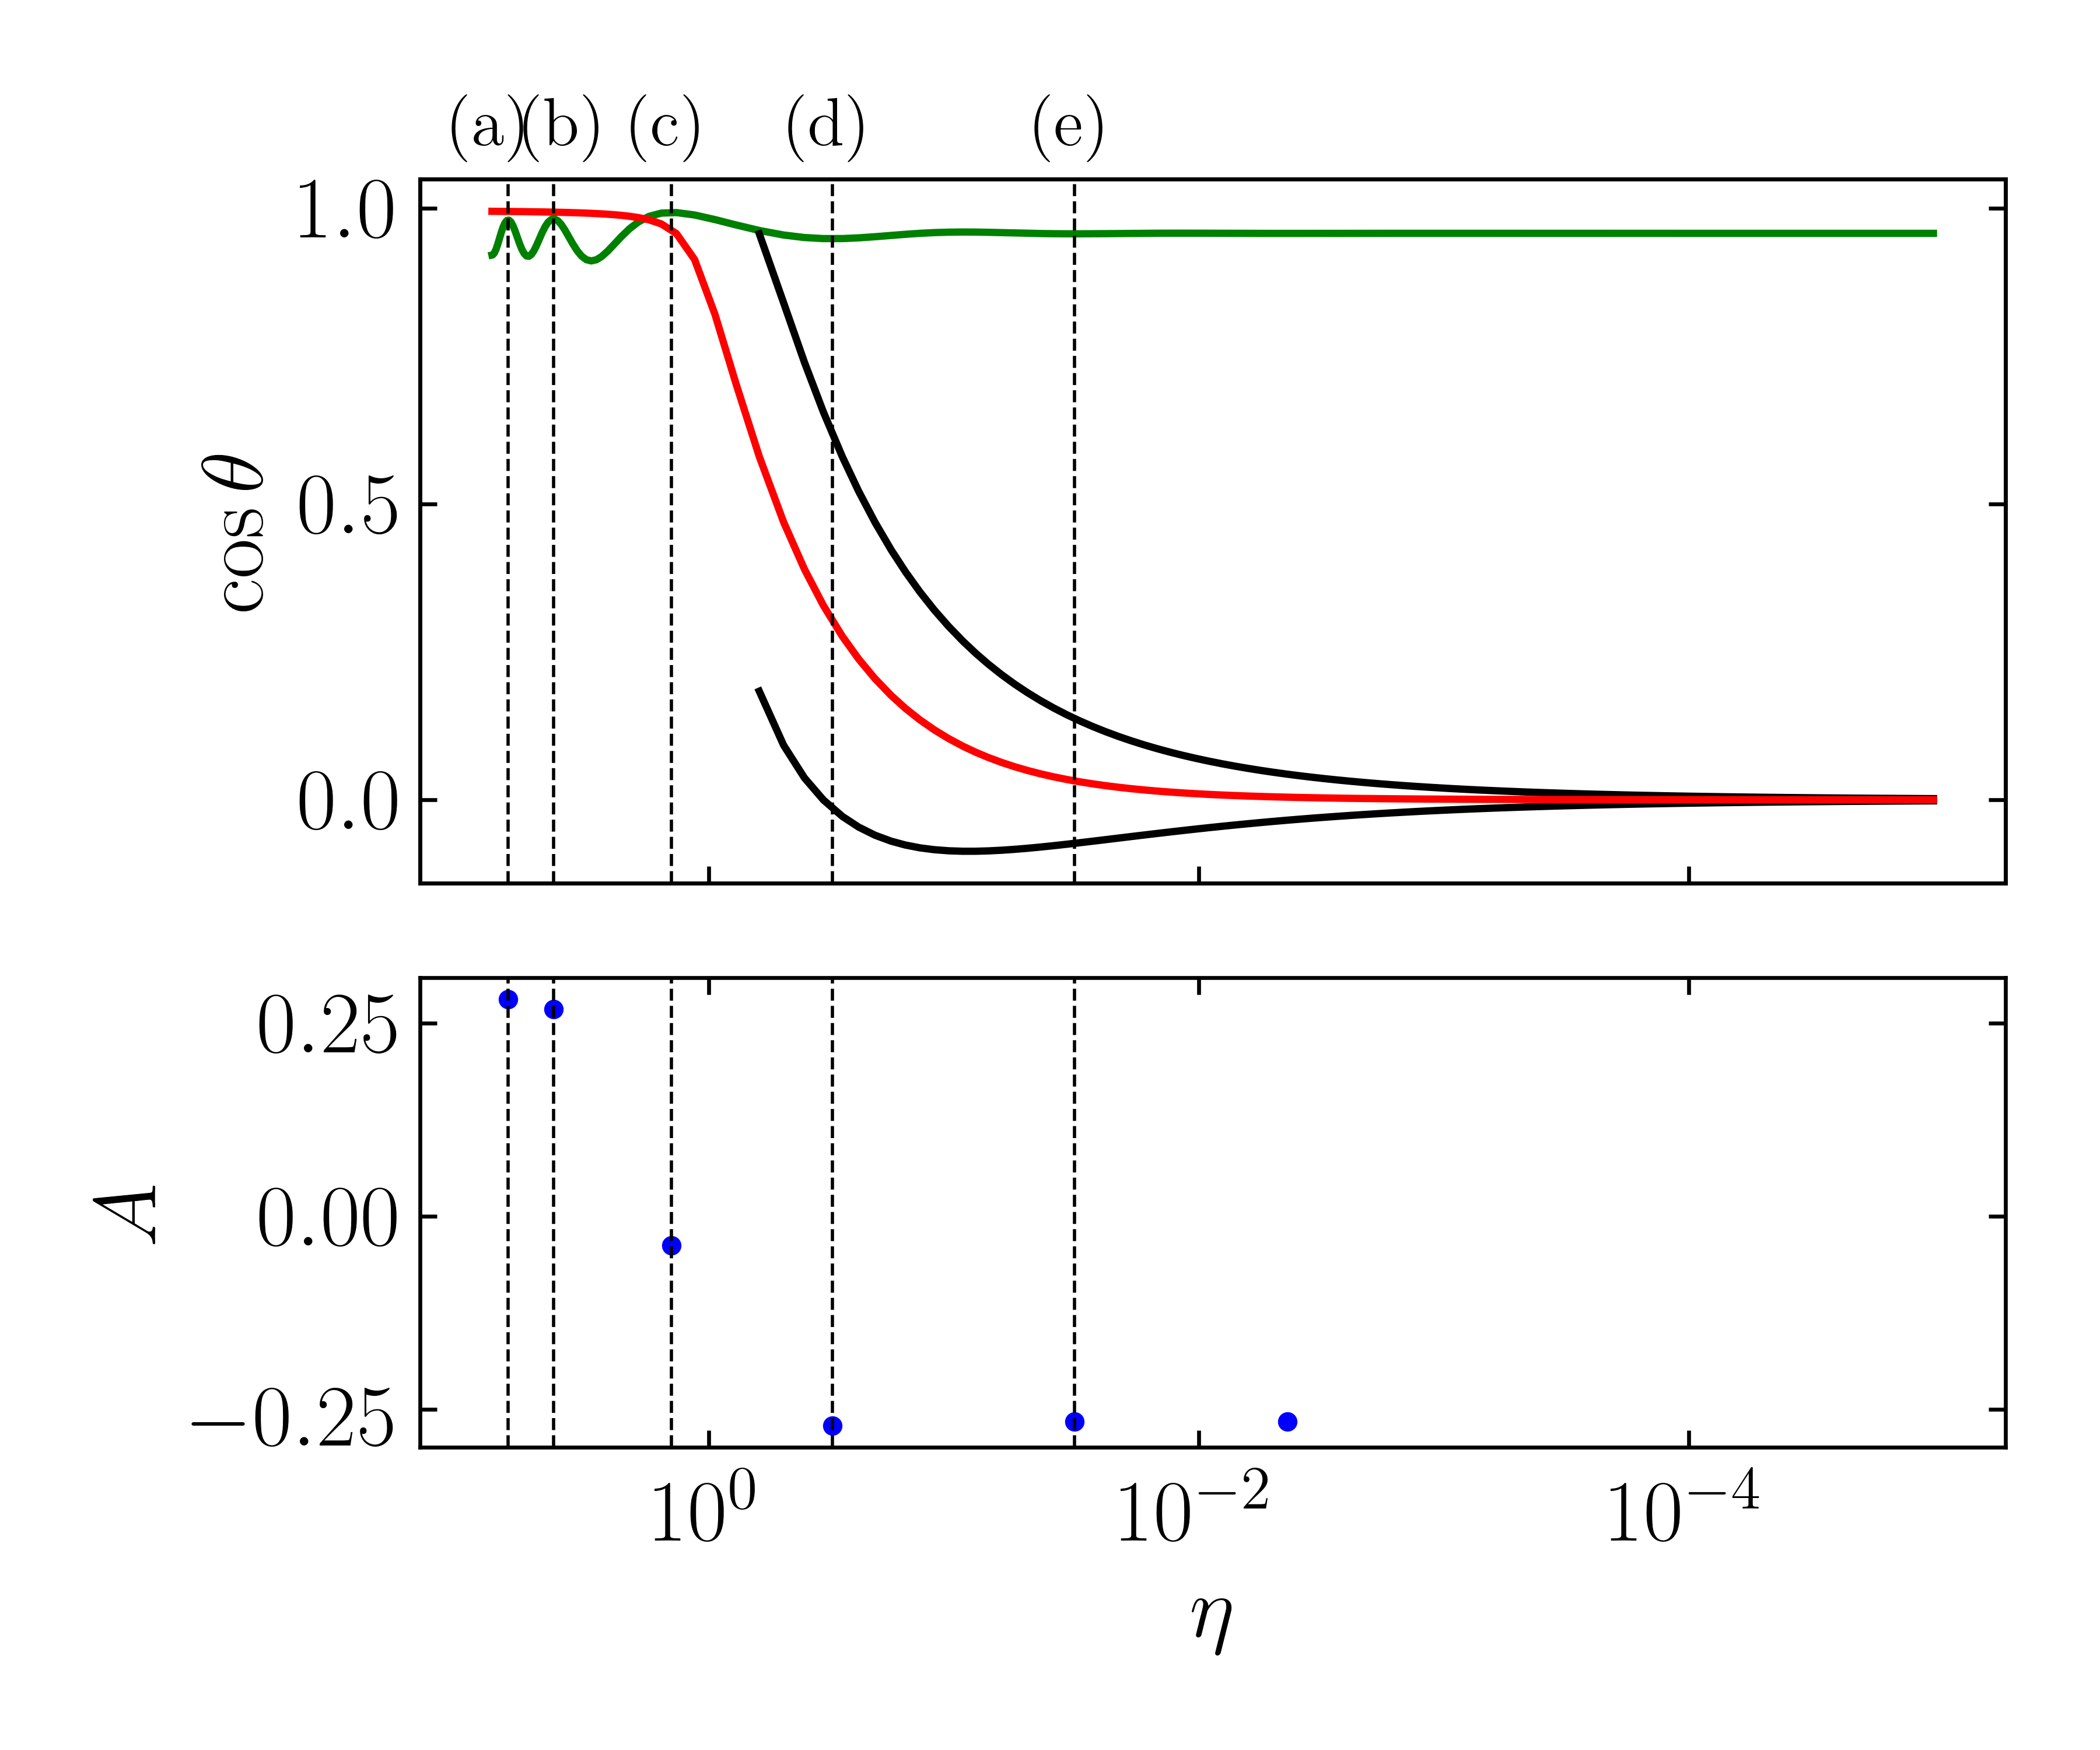
\includegraphics[width=\columnwidth]{../initial/2_toy2/3testo_nonad.png}
    \end{subfigure}
    \begin{subfigure}{\columnwidth}
        \centering
        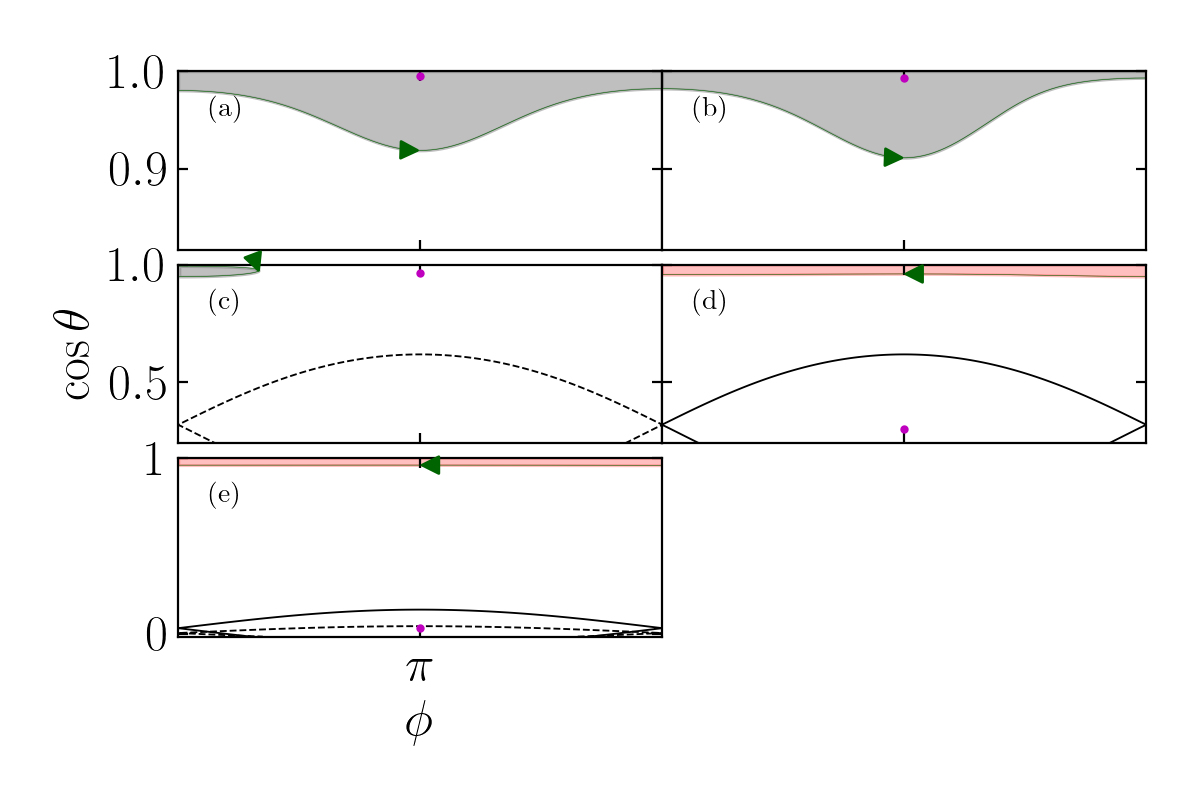
\includegraphics[width=\columnwidth]{../initial/2_toy2/3testo_nonad_subplots.png}
    \end{subfigure}
    \caption{Same as \autoref{fig:nonad_traj} but for a non-adiabatic $\epsilon =
    0.1$. In the top panel of the top plot, it is evident that the libration
    cycle about CS2 is unable to keep up with the swift motion of CS2 as $\eta$
    changes, decreasing the obliquity jump. In the bottom plot, we can see that
    individual orbits do not lie along level curves of the Hamiltonian, a
    further consequence of violating adiabaticity.}\label{fig:nonad_traj}
\end{figure}

\subsection{Dynamical Outcomes}

A formula for $\theta_{f}$ assuming $\theta_{sd, i} = 0$ initially can be
given (see \autoref{ss:app_transition})
\begin{equation}
    \theta_{f}\p{\theta_{sd, i} = 0} = \sqrt{\frac{2\pi \Omega}{\epsilon}}
        \tan I.\label{eq:nonad_q_f}
\end{equation}
We can naively generalize this by recognizing that any nonzero $\theta_{sd, i}$
manifests as obliquity variations as $\hat{s}$ librates about $\hat{l}_d$, and
these oscillations are ``frozen in'' when the disk dissipates. Thus,
\begin{equation}
    \theta_{f}\p{\theta_{sd, i}} \in \sqrt{\frac{2\pi \Omega}{\epsilon}}
        \tan I \pm \theta_{sd, i}.\label{eq:nonad_q_f_dist}
\end{equation}

We present the results of simulations for using $\epsilon = 0.3$ in
\autoref{fig:nonad_3_ensemeble}.
\begin{figure}
    \centering
    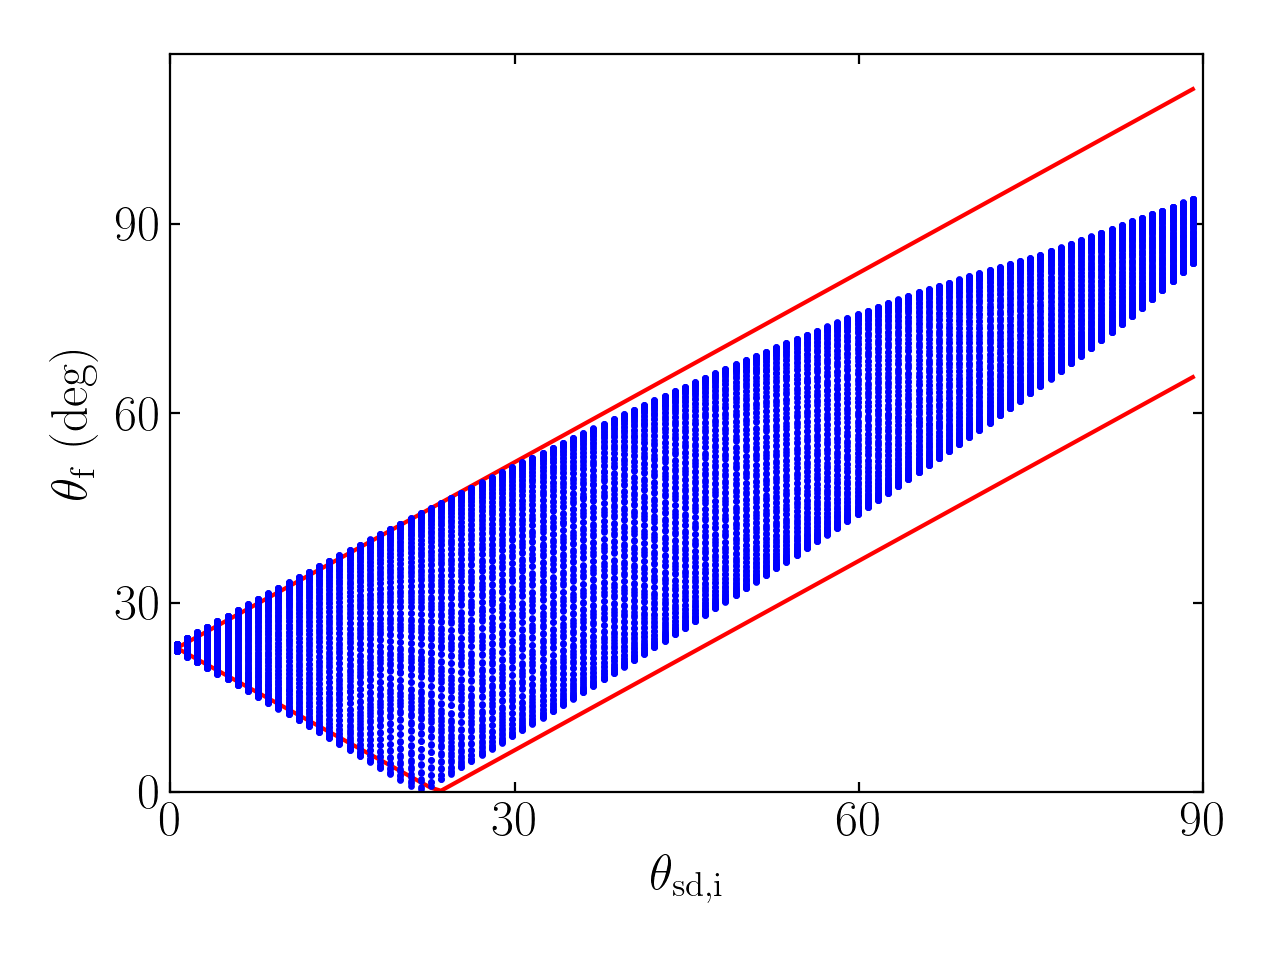
\includegraphics[width=\columnwidth]{../initial/2_toy2/3_ensemble_05_05.png}
    \caption{$\theta_{ f}\p{\theta_{sd, i}}$ at $\epsilon = 0.3$, firmly in
    the non-adiabatic regime. Note the clear double-valuedeness has disappeared,
    as have distinct dynamical tracks. The red dotted line presents the
    analytical prediction given by
    \autoref{eq:nonad_q_f_dist}.}\label{fig:nonad_3_ensemeble}
\end{figure}

The agreement of \autoref{eq:nonad_q_f} at fixed $I$ for varying $\epsilon$ is
shown in \autoref{fig:nonad_3_scan}. Note that $\epsilon \to 0$ recovers the
adiabatic regime.
\begin{figure}
    \centering
    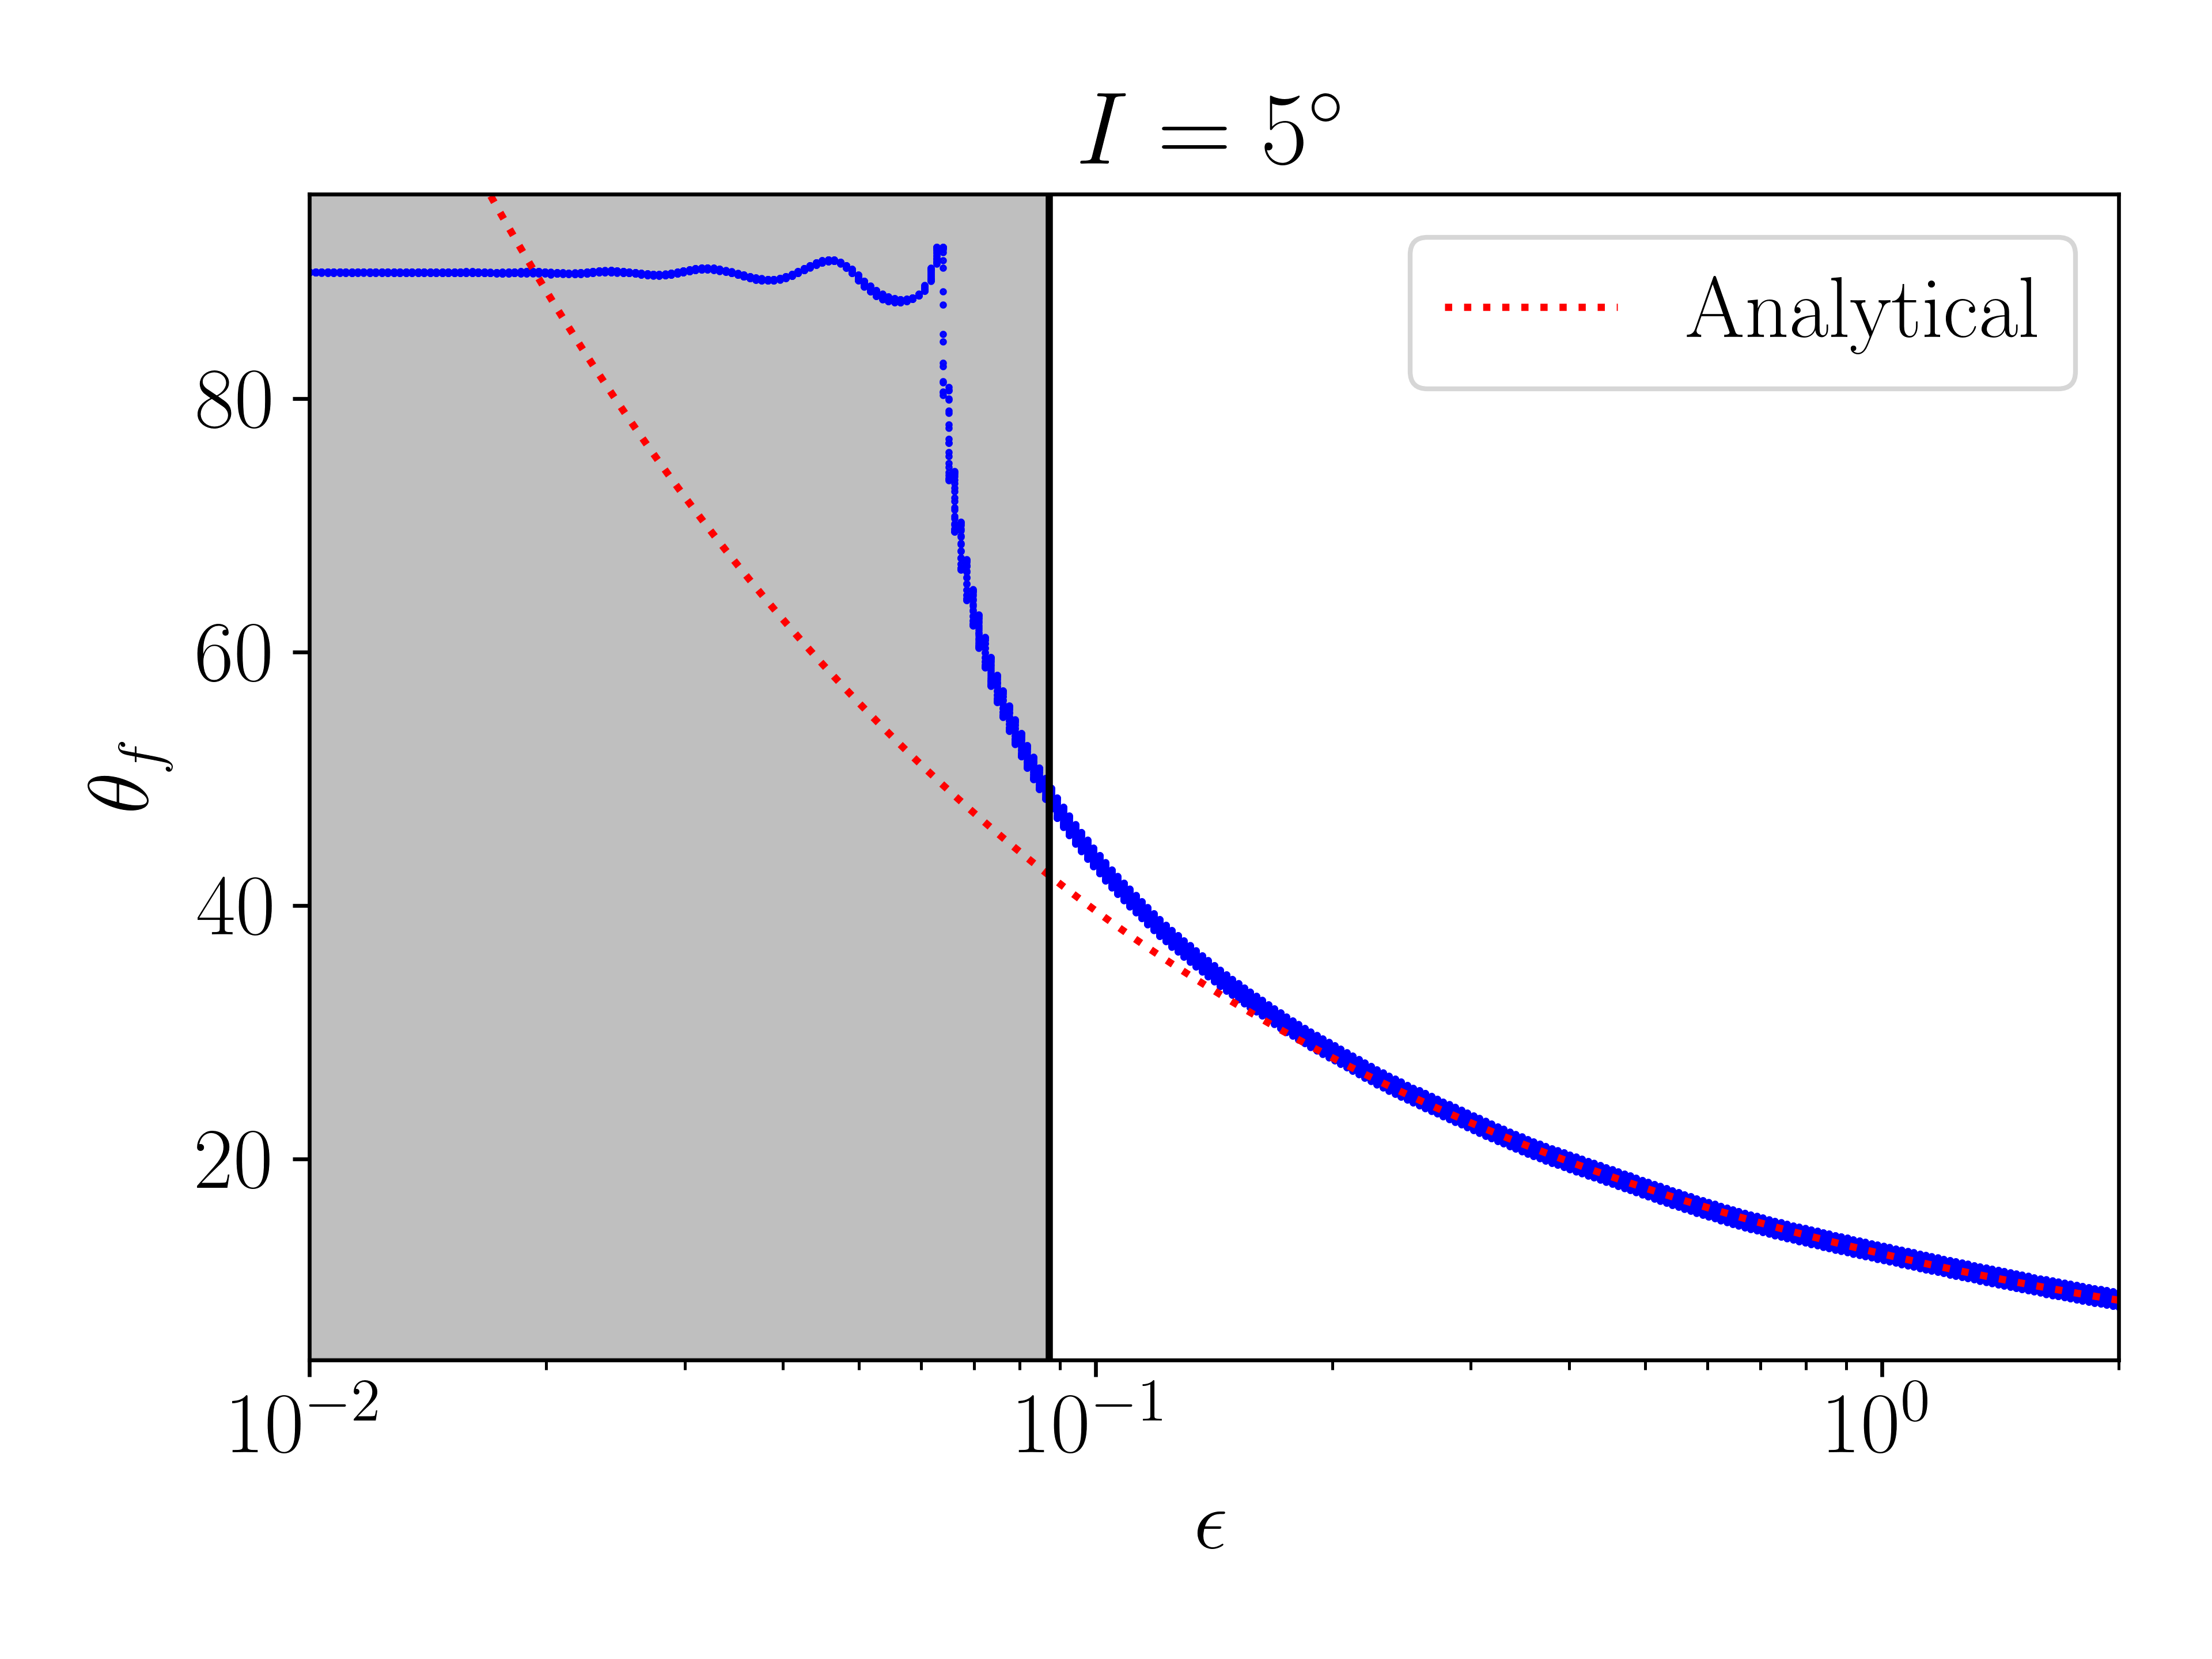
\includegraphics[width=\columnwidth]{../initial/2_toy2/3scan.png}
    \caption{Plot of $\theta_{ f}\p{\theta_{sd, i} = 0}$ as a function of
    $\epsilon$, where $I = 5^\circ$. Overplotted in the red line is
    \autoref{eq:nonad_q_f}, which is in good agreement for $\epsilon \gtrsim
    0.1$ the non-adiabatic regime, while $\theta_{ f} \approx 90^\circ$ in
    the adiabatic regime.}\label{fig:nonad_3_scan}
\end{figure}

\bibliographystyle{mnras}
\bibliography{Su_sep_cross}

% \clearpage
% \onecolumn
\appendix

\section{Adiabatic Evolution}

\subsection{Adiabatic Dynamical Histories}\label{ss:app_tracks}

\begin{itemize}
    \item $A_{II} \to A_{I}$ --- \autoref{fig:ad_21}.
    \item $A_{II} \to A_{III}$ --- \autoref{fig:ad_23}.
    \item $A_{III} \to A_{I}$ --- \autoref{fig:ad_31}.
    \item $A_{III} \to A_{II} \to A_{I}$ --- \autoref{fig:ad_321}.
    \item $A_{III} \to A_{III}$ --- Trivial case, the initial enclosed area is
        too large to ever experience a separatrix encounter.
\end{itemize}
\begin{figure}
    \centering
    \begin{subfigure}{\columnwidth}
        \centering
        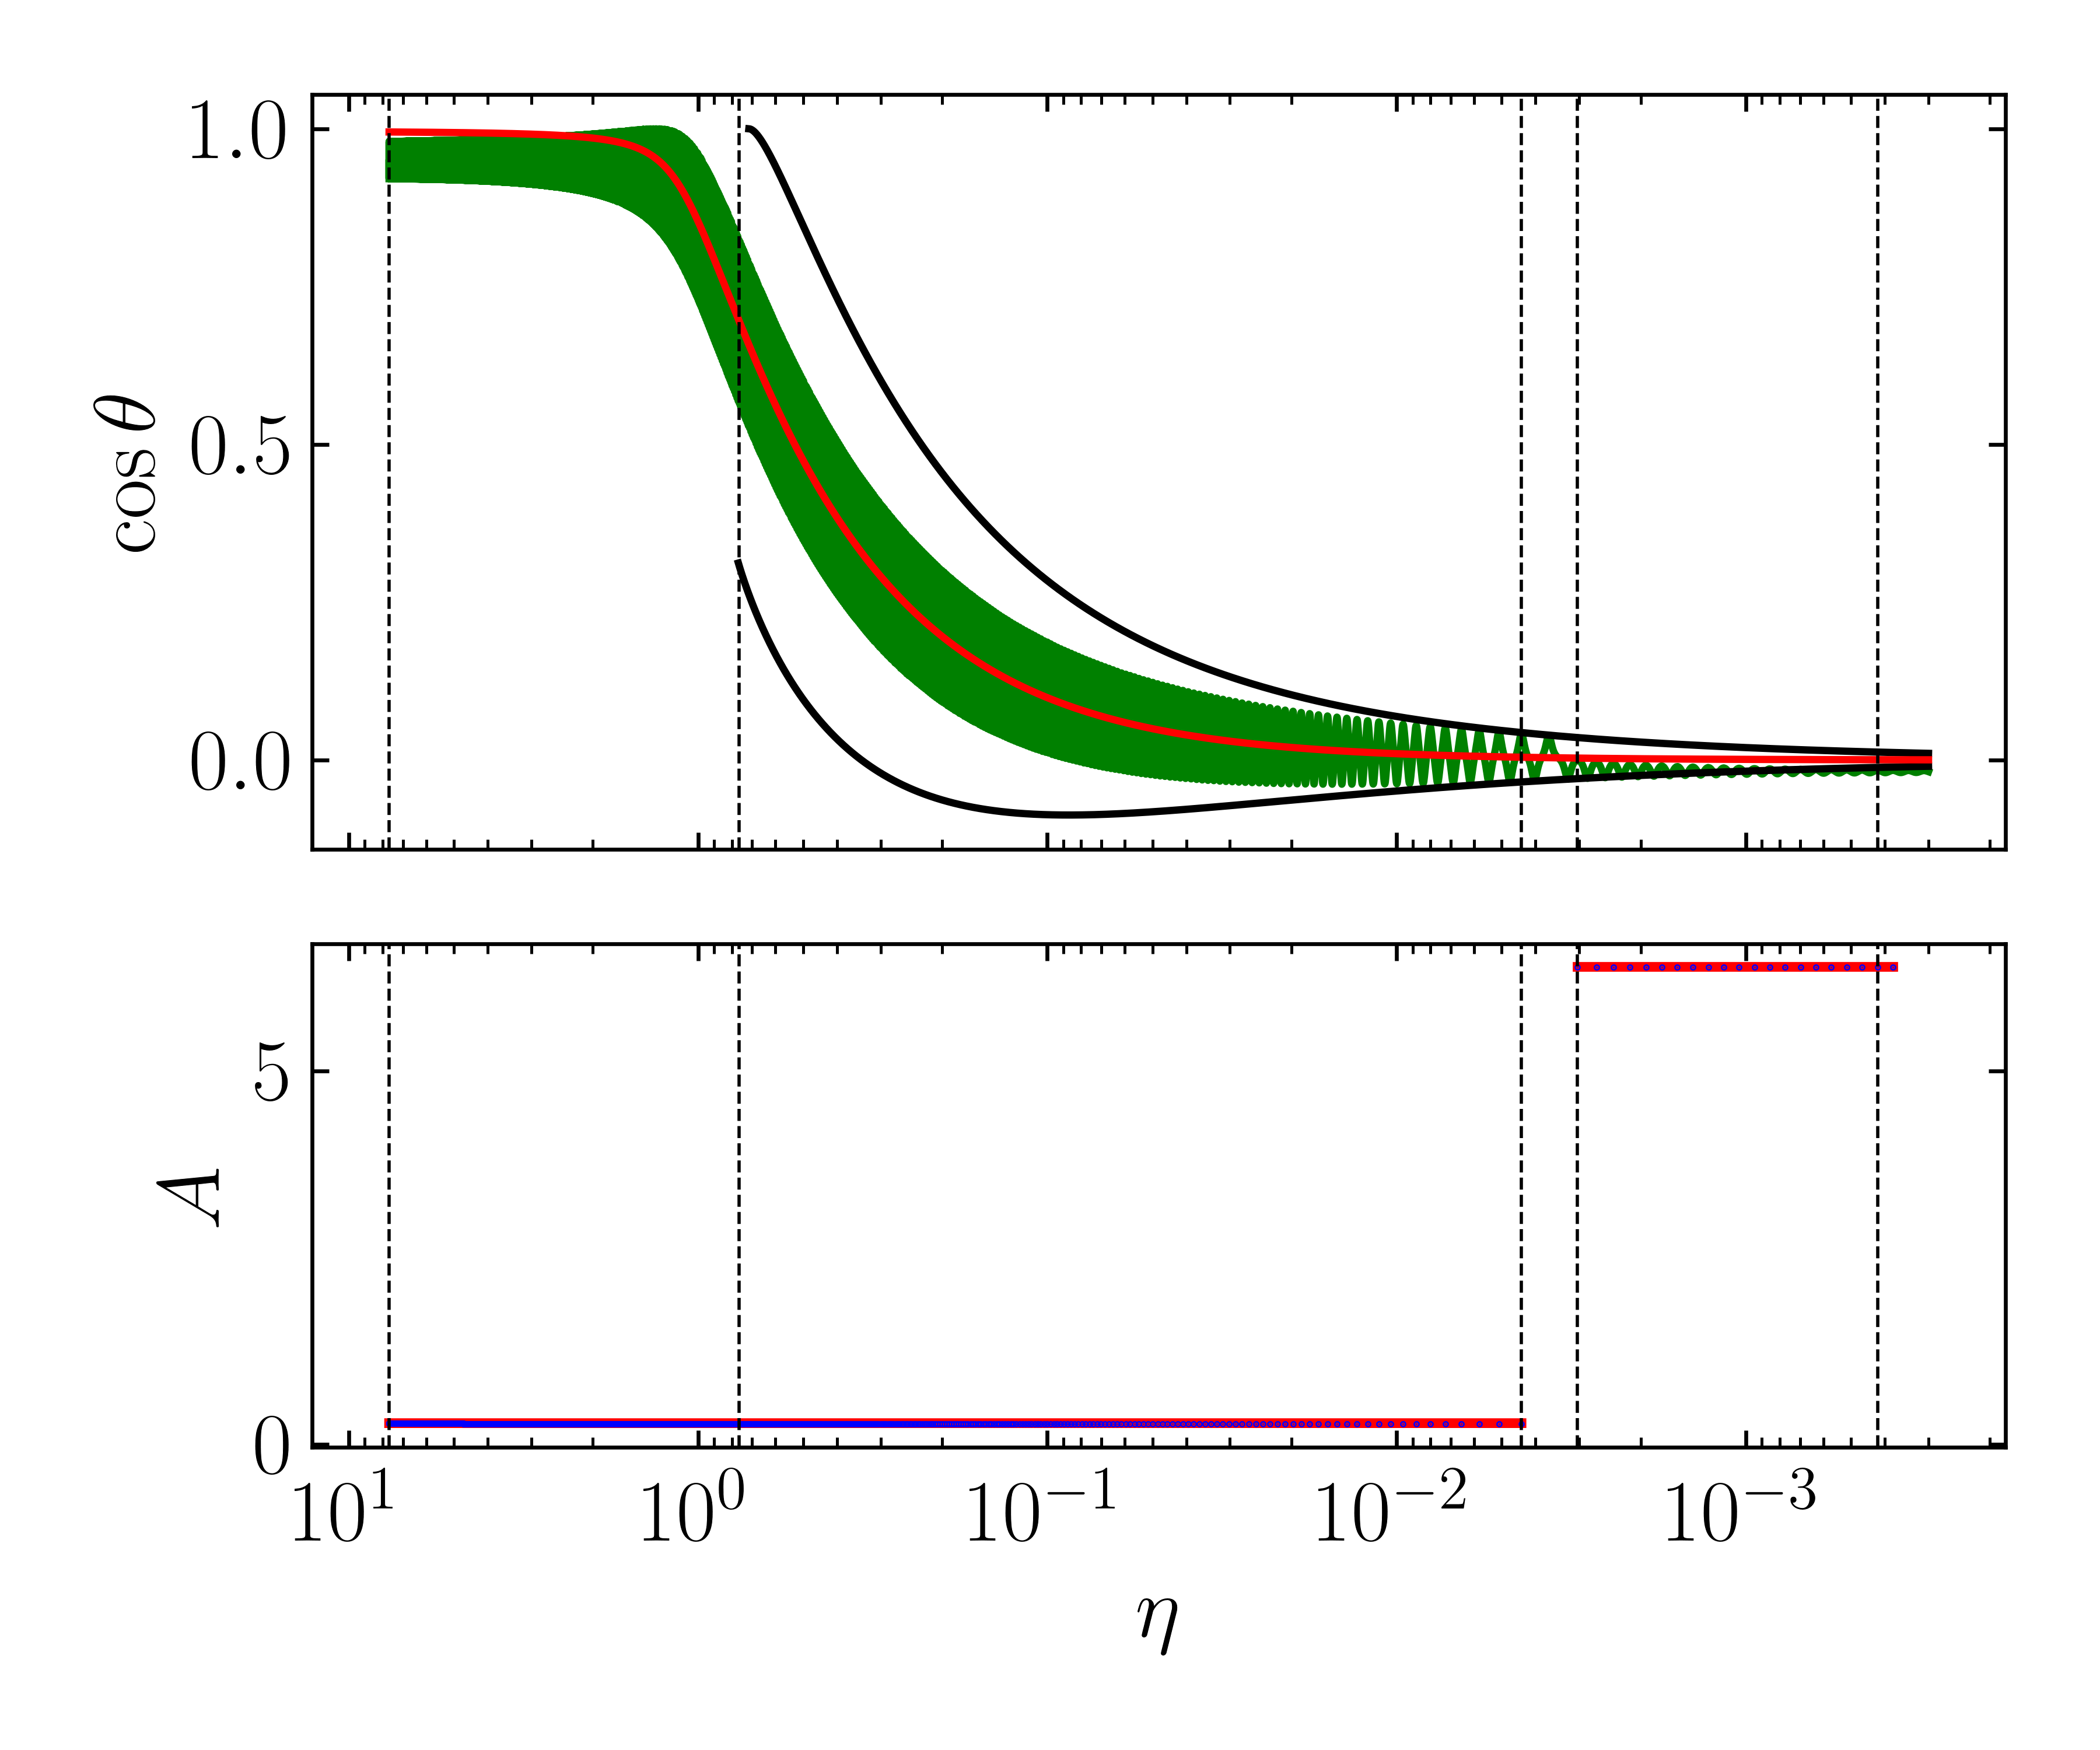
\includegraphics[width=\columnwidth]{../initial/2_toy2/3testo23.png}
    \end{subfigure}
    \begin{subfigure}{\columnwidth}
        \centering
        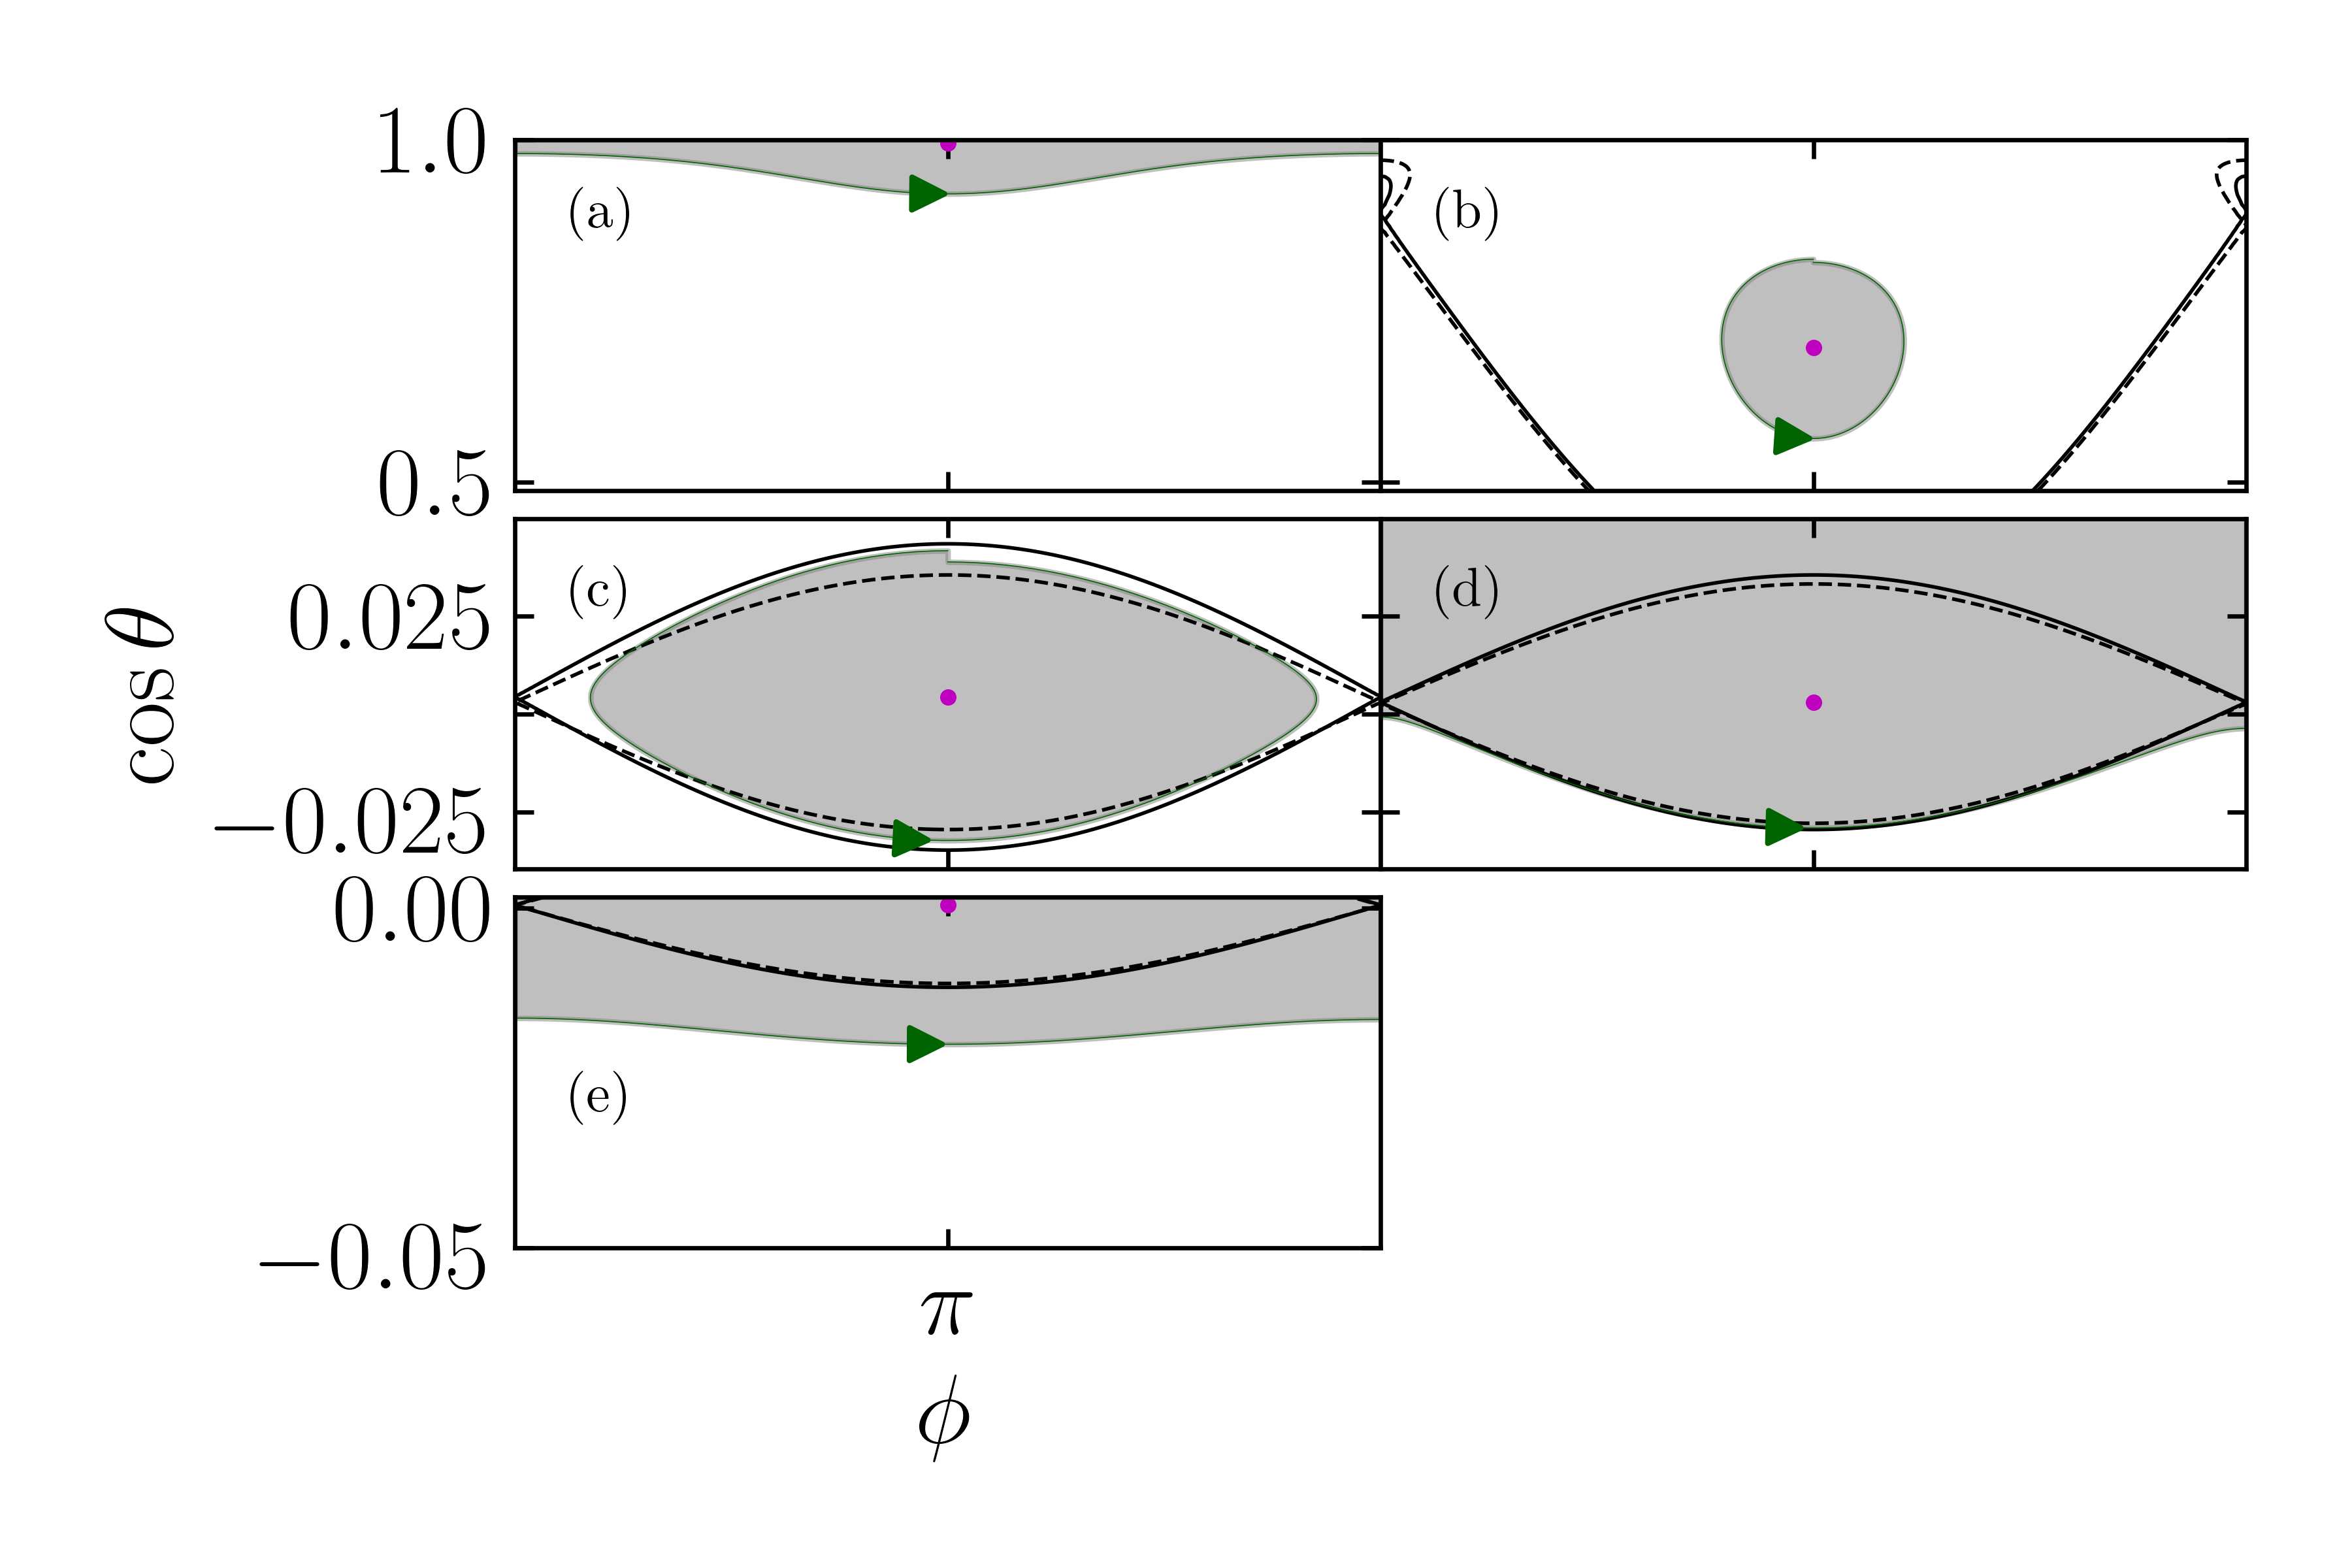
\includegraphics[width=\columnwidth]{../initial/2_toy2/3testo23_subplots.png}
    \end{subfigure}
    \caption{Same as \autoref{fig:ad_21} but for the $A_2 \to A_3$ track.
    }\label{fig:ad_23}
\end{figure}
\begin{figure}
    \centering
    \begin{subfigure}{\columnwidth}
        \centering
        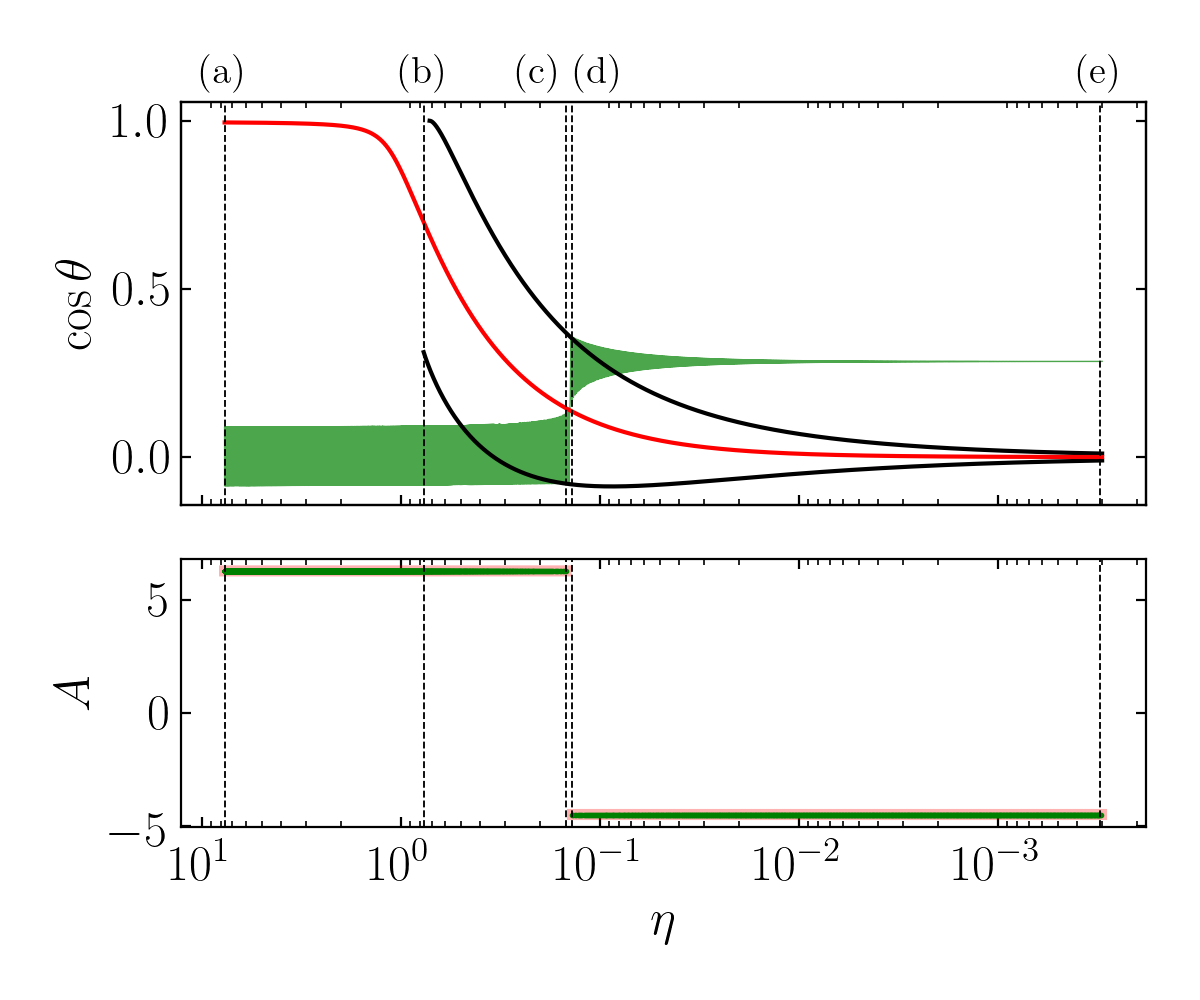
\includegraphics[width=\columnwidth]{../initial/2_toy2/3testo31.png}
    \end{subfigure}
    \begin{subfigure}{\columnwidth}
        \centering
        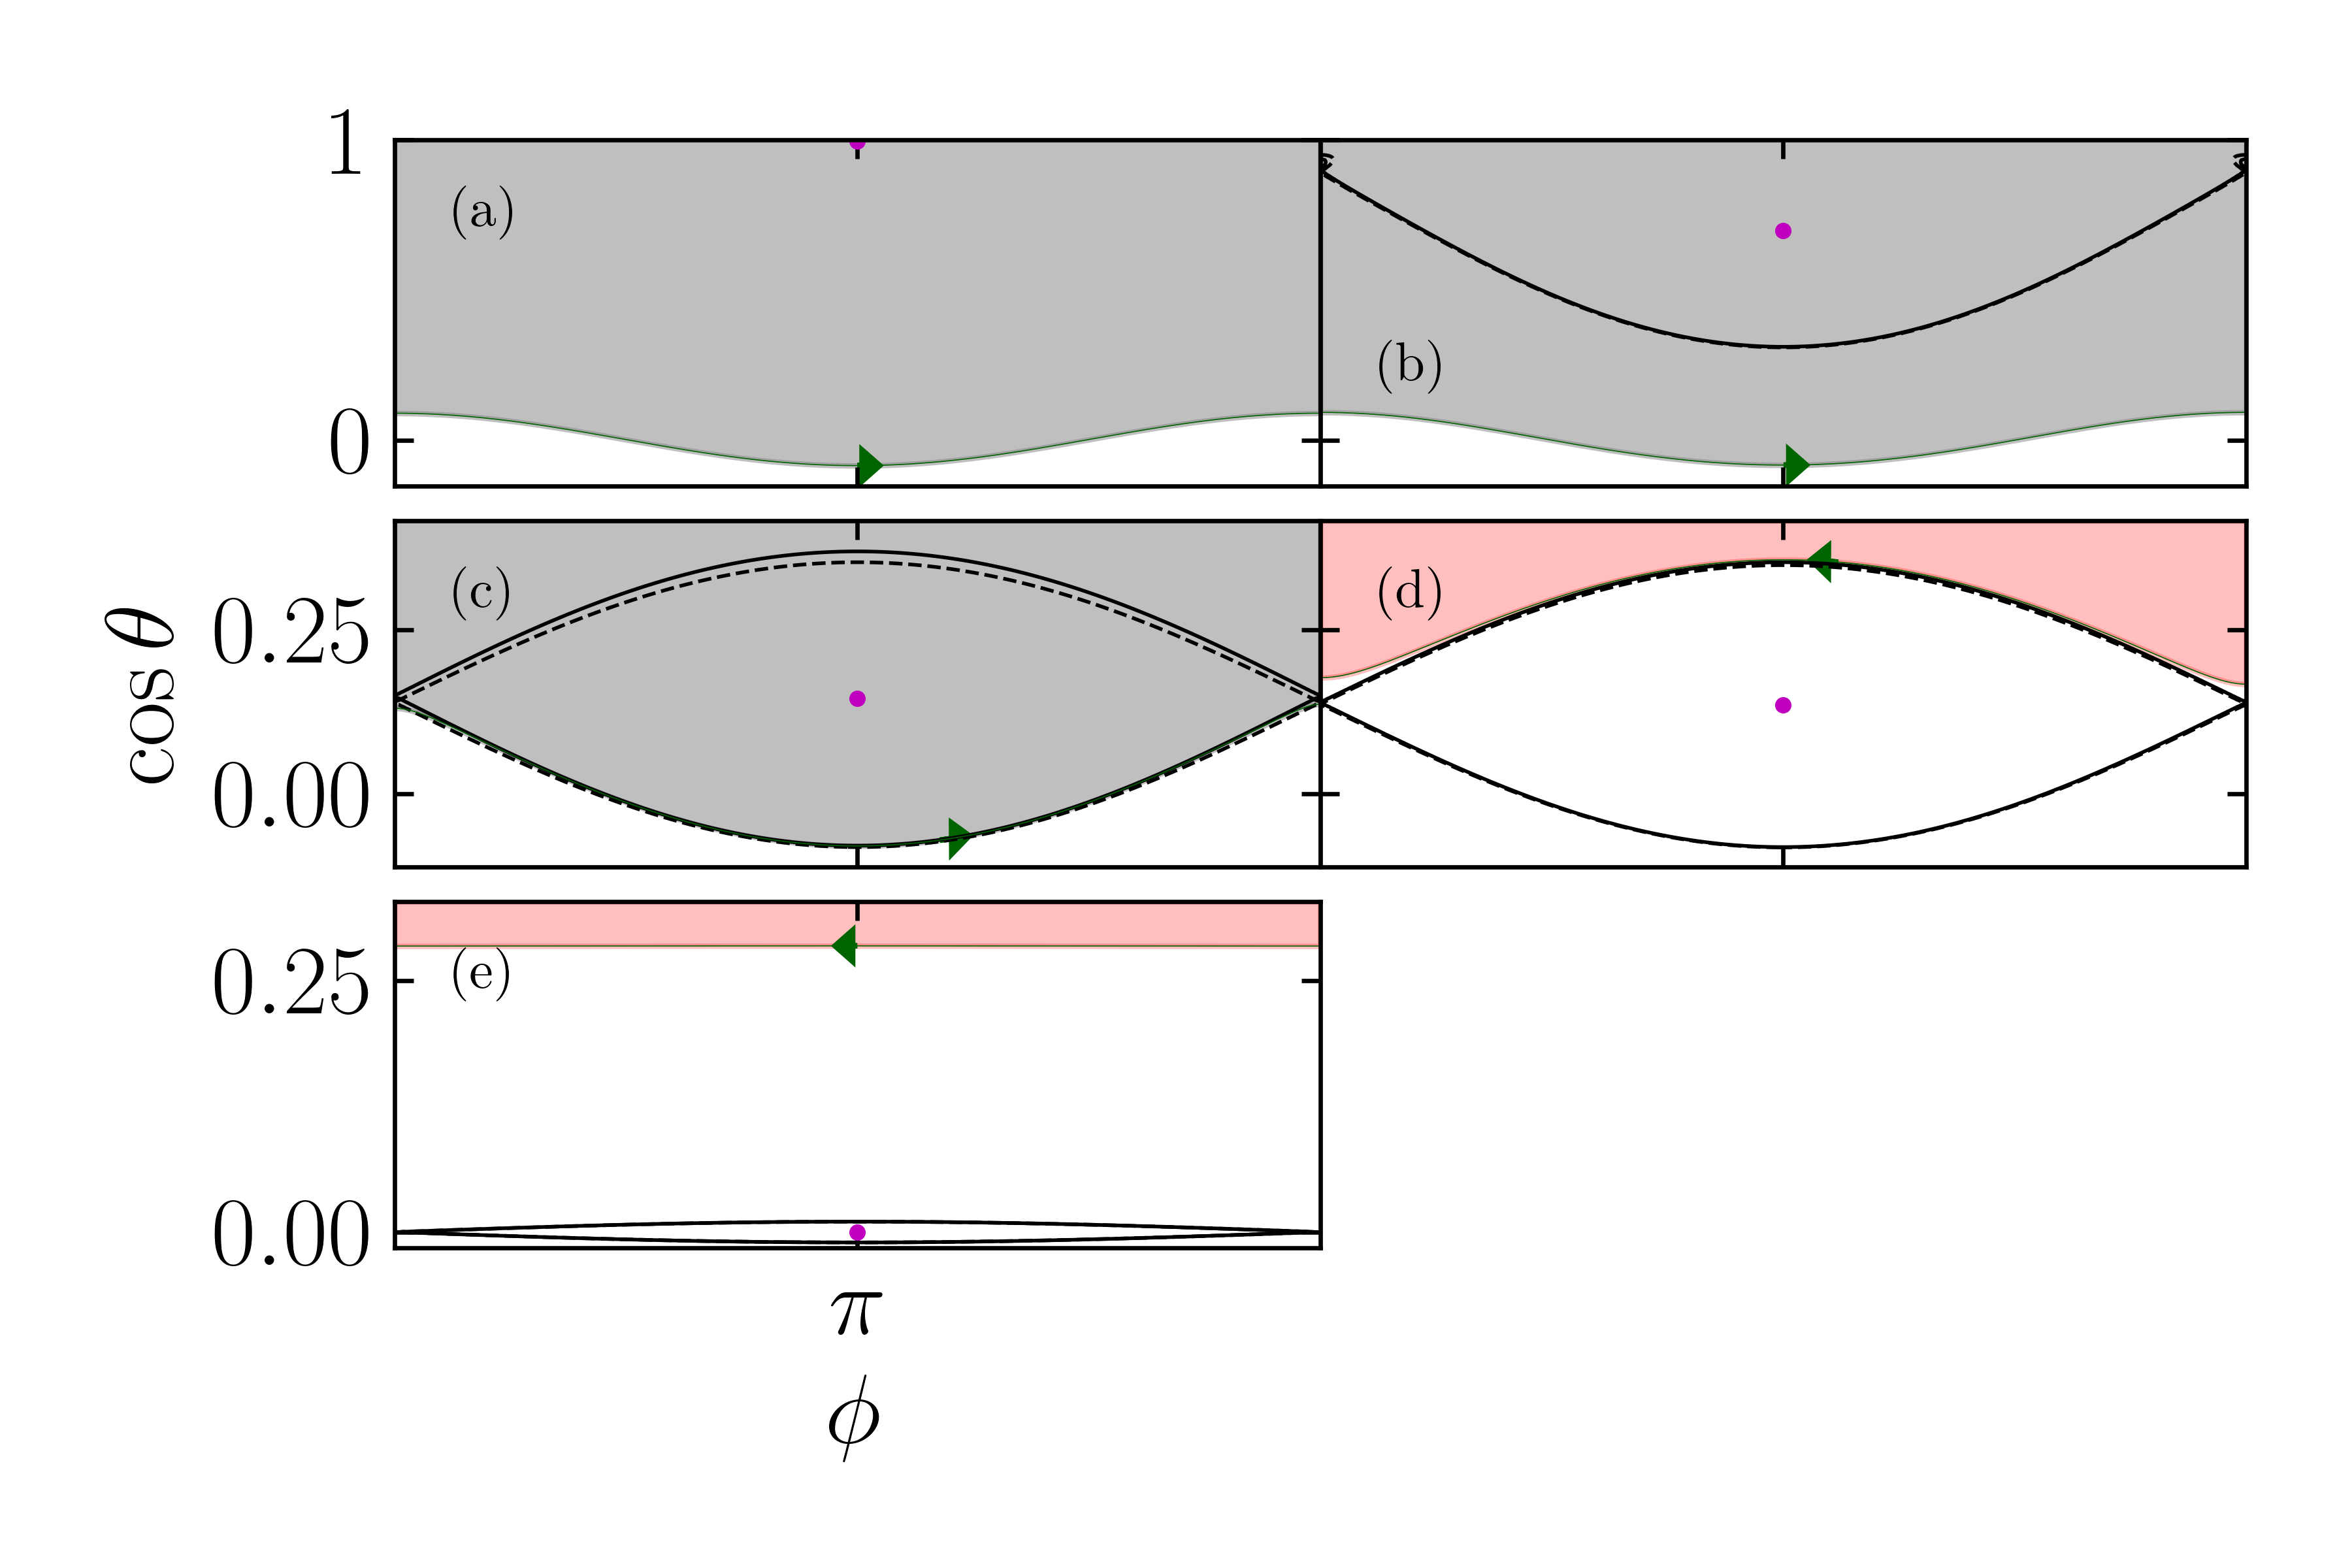
\includegraphics[width=\columnwidth]{../initial/2_toy2/3testo31_subplots.png}
    \end{subfigure}
    \caption{Same as \autoref{fig:ad_21} but for the $A_{III} \to A_I$
    track.}\label{fig:ad_31}
\end{figure}
\begin{figure}
    \centering
    \begin{subfigure}{\columnwidth}
        \centering
        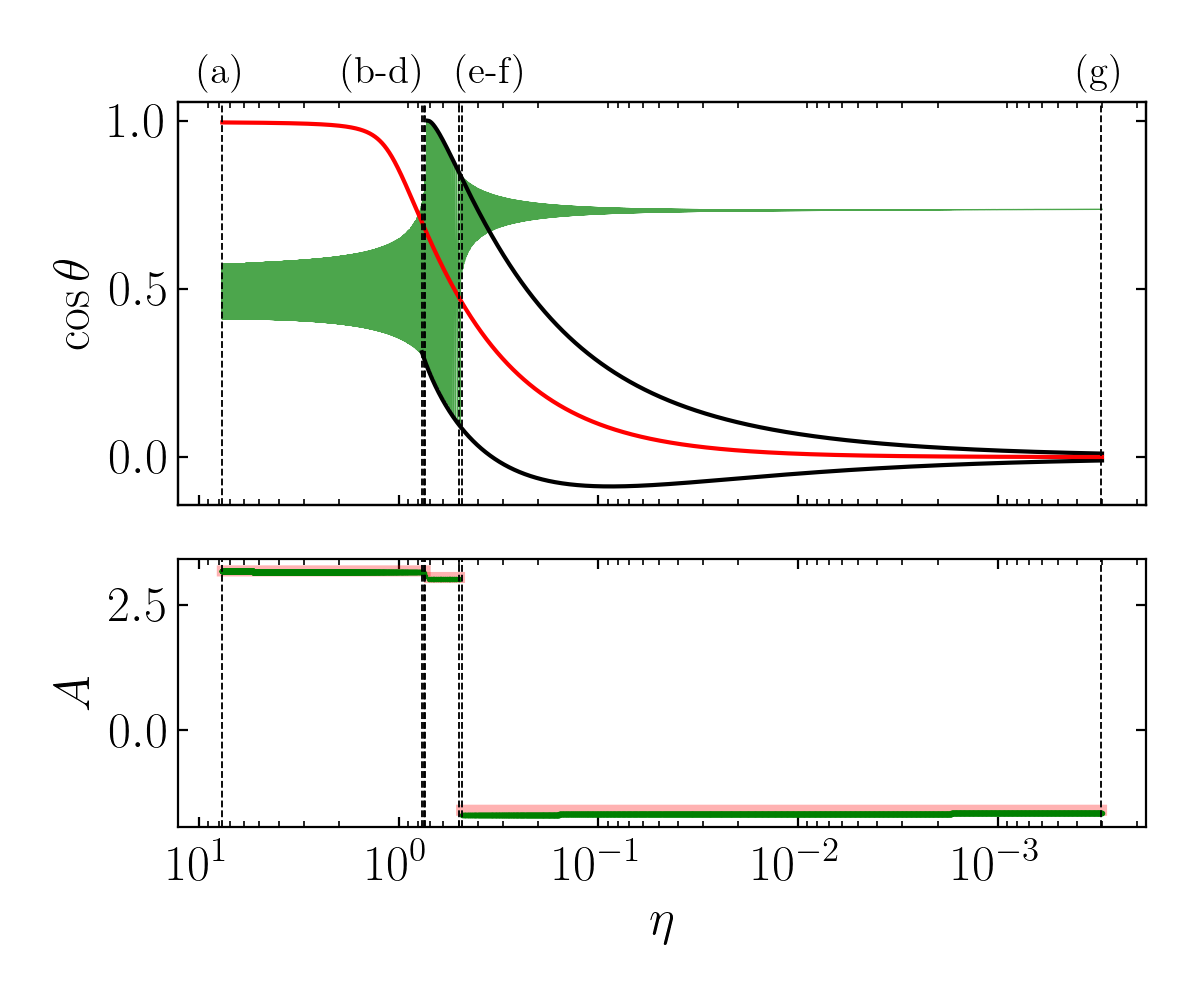
\includegraphics[width=\columnwidth]{../initial/2_toy2/3testo321.png}
    \end{subfigure}
    \begin{subfigure}{\columnwidth}
        \centering
        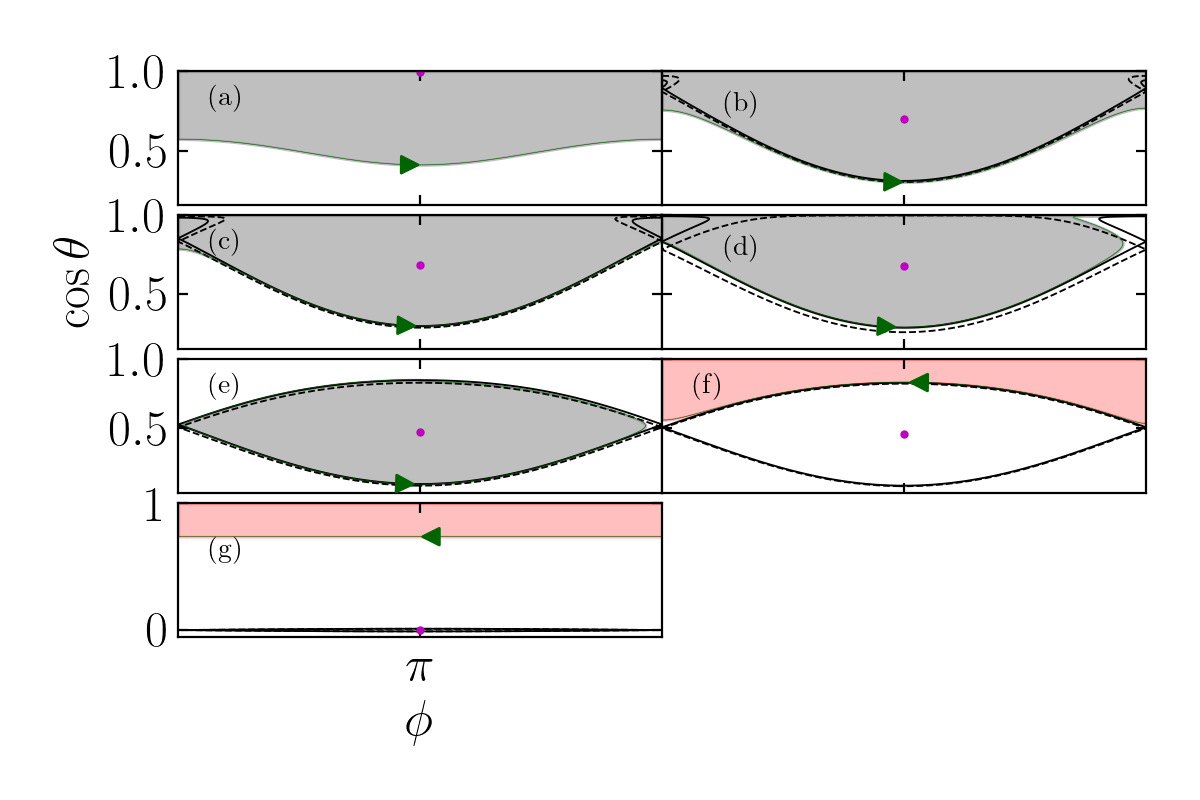
\includegraphics[width=\columnwidth]{../initial/2_toy2/3testo321_subplots.png}
    \end{subfigure}
    \caption{Same as \autoref{fig:ad_21} but for the $A_{III} \to A_{II} \to A_I$
    track. Two separatrix crossings are shown.}\label{fig:ad_321}
\end{figure}

\subsection{Adiabatic Tracks at Varying $I$}\label{ss:varying_I}

See \autoref{fig:varying_i}.
\begin{figure}
    \centering
    \begin{subfigure}{\columnwidth}
        \centering
        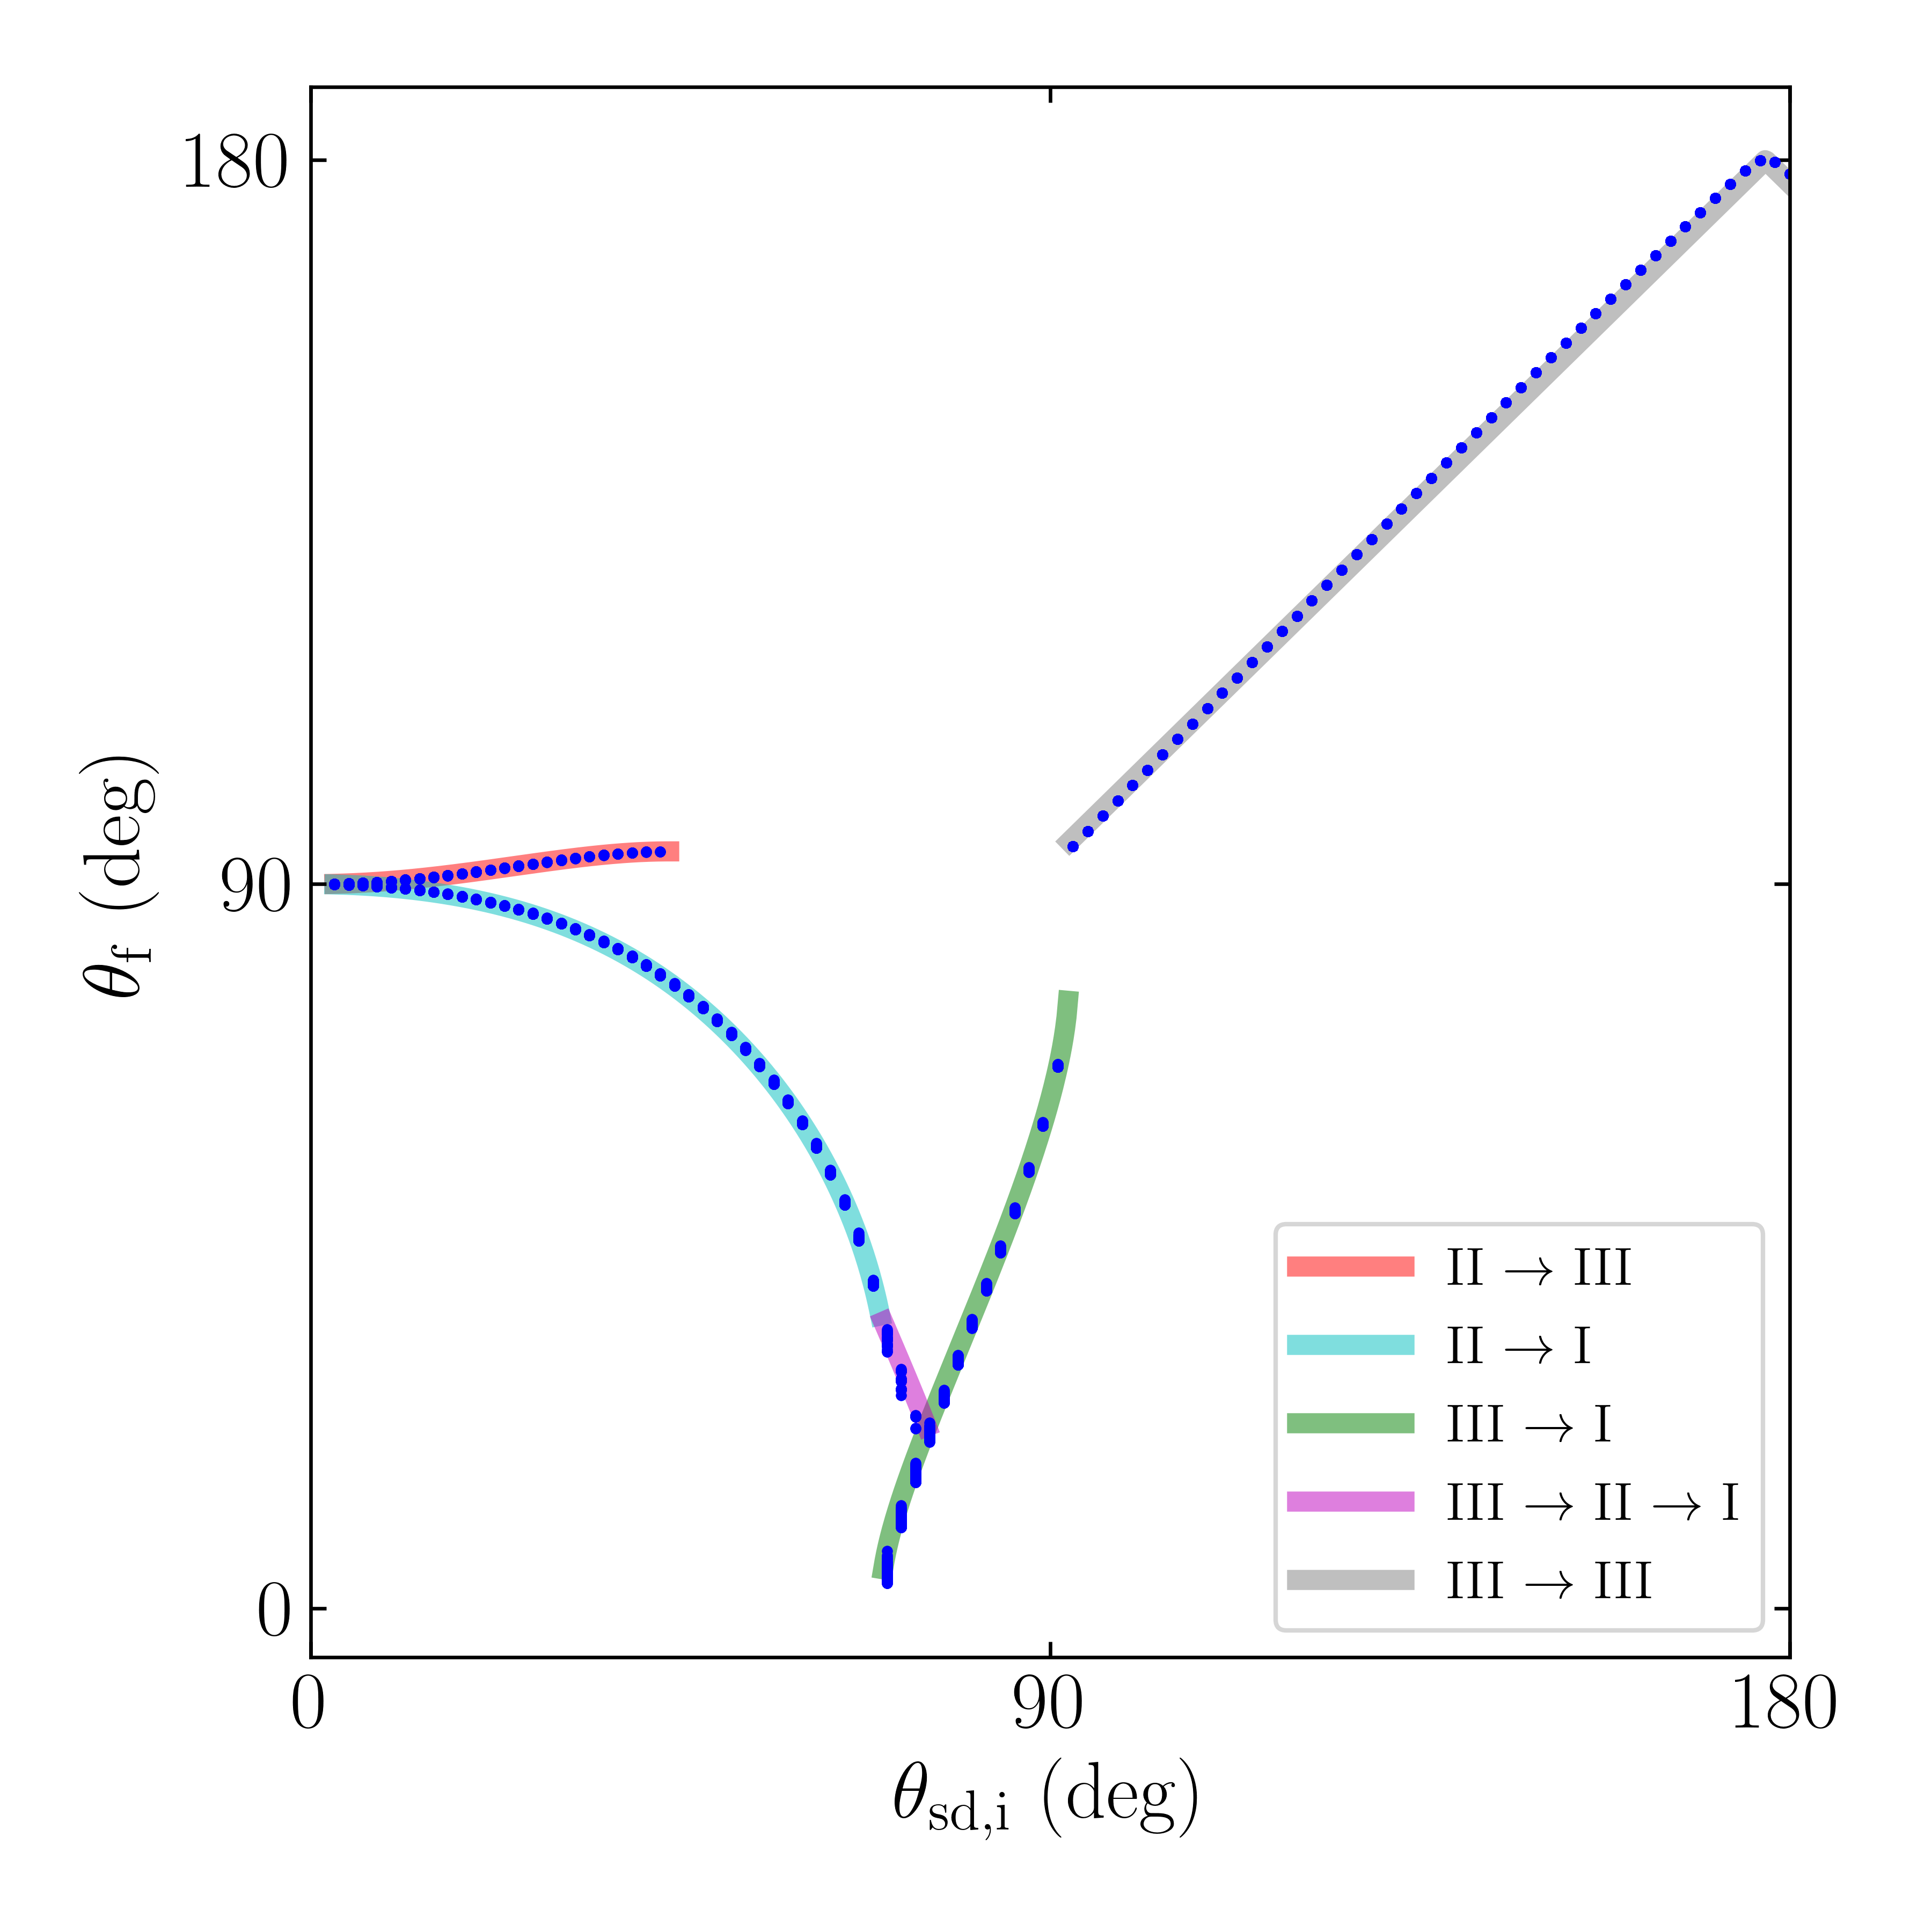
\includegraphics[width=\columnwidth]{../initial/2_toy2/3_ensemble_10_35.png}
    \end{subfigure}
    \begin{subfigure}{\columnwidth}
        \centering
        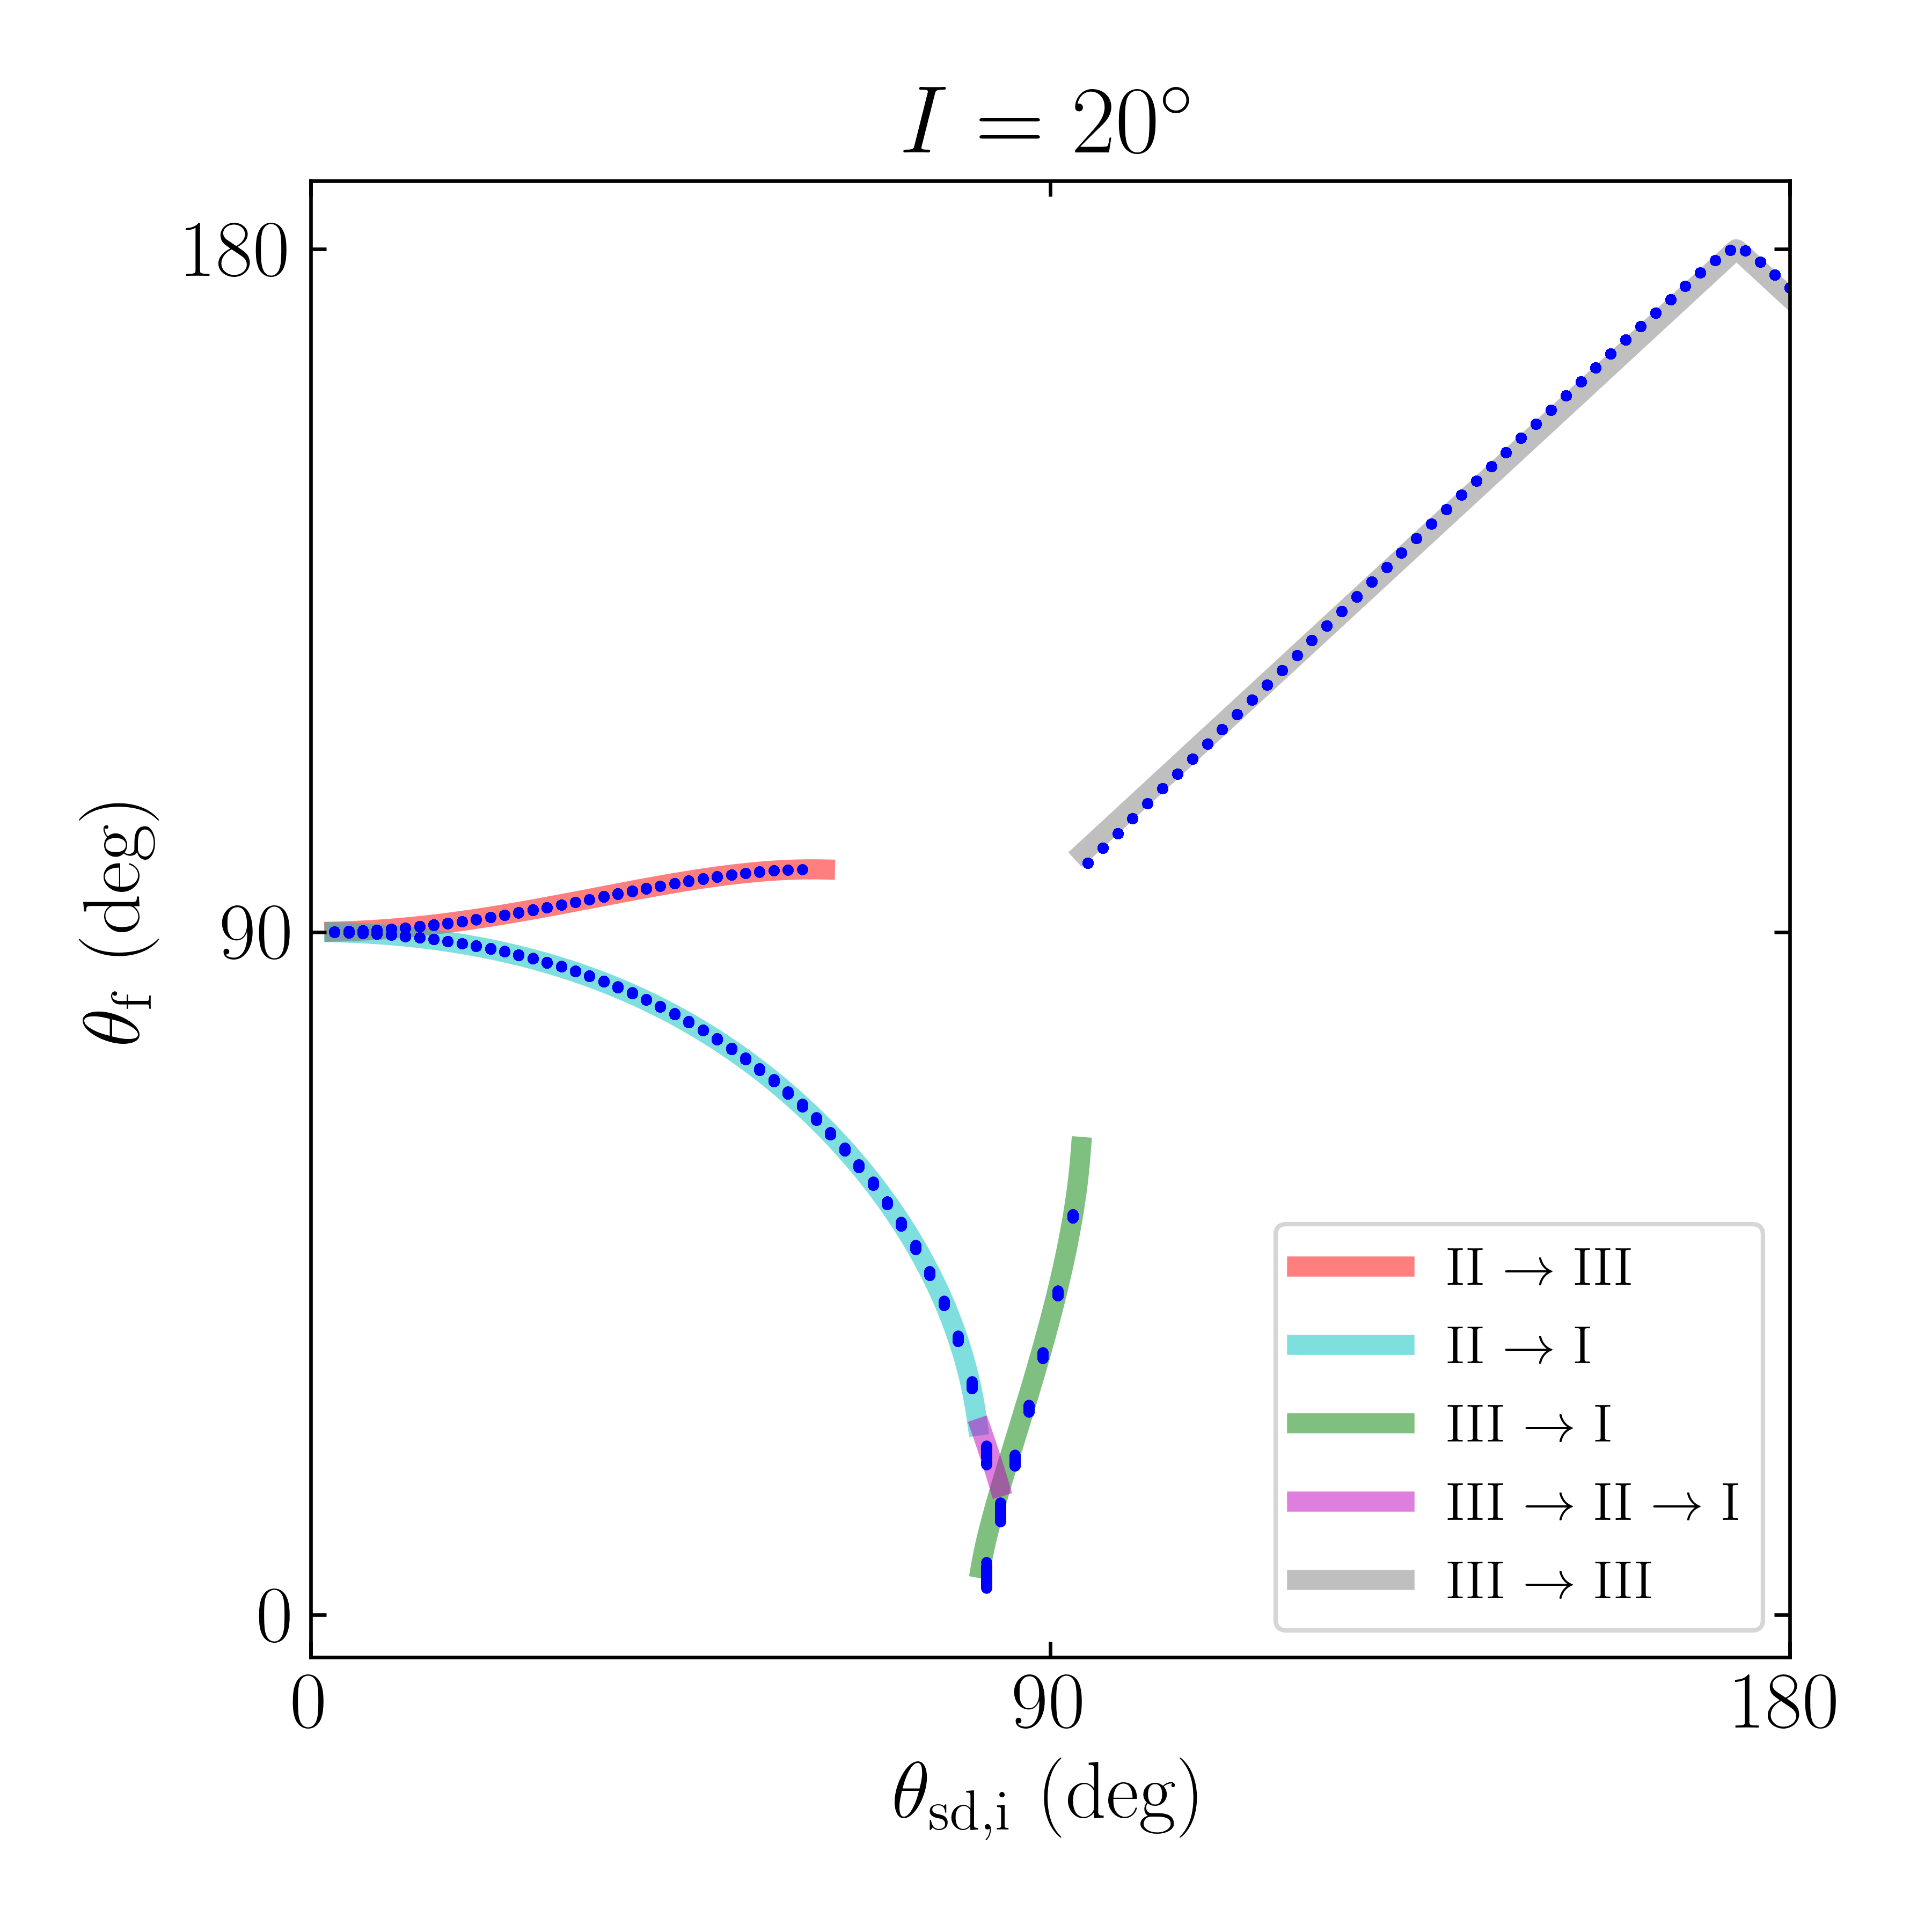
\includegraphics[width=\columnwidth]{../initial/2_toy2/3_ensemble_20_35.png}
    \end{subfigure}
    \caption{Same as \autoref{fig:ad_ensemble} but for $I = 10^\circ$ (top) and
    $I = 20^\circ$ (bottom).}\label{fig:varying_i}
\end{figure}

\subsection{$\theta_f$ for Adiabatic Tracks}\label{ss:app_transition}

To understand how trajectories transition between zones, we must recall the
result from \citep{henrard1982,henrard1987}: if a zone $i$ is shrinking and zone
$j$ is expanding, the probability of transition from zone $i$ to zone $j$ is
given
\begin{equation}
    \Pr_{i \Rightarrow j} = -\frac{\pd{A_j}{t}}{ \pd{A_i}{t}}
        = -\frac{\pd{A_j}{\eta}}{ \pd{A_i}{\eta}}\label{eq:henrard_hop}
\end{equation}
This can be used directly in conjunction with \autoref{se:area_ward} to generate
the probabilities in the bottom panel of \autoref{fig:ad_ensemble}.

Next, we will compute an approximate closed form for the final obliquities for
the initial conditions in zone II (which experience separatrix crossing at
$\eta_\star \ll 1$), we first seek a simple parameterization for the separatrix.
We first solve for equilibria of the equation of motion \autoref{eq:dsdt_base}
to compute the coordinates for Cassini State 4:
\begin{equation}
    \cos \theta_4 \approx \frac{\mu \cos I}{1 - \eta \sin I}.
\end{equation}
Note that $\phi_4 = 0$. Then, the separatrix is the level curve of the
Hamiltonian intersecting CS4, so it satisfies $H\p{\theta_{sep}(\phi), \phi} =
H\p{\theta_4, \phi_4}$. This solves to be approximately
\begin{equation}
    \cos \theta_{sep}(\phi) \approx \cos \theta_4 \pm
        \sqrt{2\eta \sin I\p{1 - \cos \phi}}.
\end{equation}
Integration of the phase area enclosed by the two legs of the separatrix then
yields
\begin{equation}
    A_{II}(\eta) \approx 16\sqrt{\eta \sin I}.\label{eq:a_approx}
\end{equation}
This, in conjunction with \autoref{eq:henrard_hop}, is sufficient to compute
$\theta_f\p{\theta_{sd, i}}$ for zone II initial conditions.

\begin{itemize}
    \item For a given $\theta_{sd, i}$, we know that if $\eta \to \infty$ then
        the trajectory executes simple libration about $\hat{l}_d$, and so $A =
        2\pi\p{1 - \cos \theta_{sd, i}} \approx \pi \theta_{sd, i}^2$. This
        then implies $\eta_\star$ must be the solution to $A_{II}(\eta_\star) =
        A$, or
        \begin{align}
            \eta_\star &\approx \p{\frac{2\pi\p{1 - \cos \theta_{sd,i}}}{
                        16}}^2 / \sin I,\nonumber\\
                    &\approx \p{\frac{\pi \theta_{sd, i}^2}{16}}^2/\sin I.
        \end{align}

    \item Upon separatrix encounter, a transition to either zone I or zone III
        occurs. These can be calculated to have associated probabilities (using
        the approximate area \autoref{eq:a_approx})
        \begin{align}
            \Pr_{II \Rightarrow I} &\approx \frac{2\pi
                \eta_{\star} \cos I + 4\sqrt{\eta_{\star}\sin
                I}}{8\sqrt{\eta_{\star}\sin I}},\\
            \Pr_{II \Rightarrow III} &\approx \frac{-2\pi
                \eta_{\star} \cos I + 4\sqrt{\eta_{\star}\sin
                I}}{8\sqrt{\eta_{\star}\sin I}}.
        \end{align}

    \item Upon a transition to zone I or zone III, the final obliquities can be
        predicted by observing the final adiabatic invariant $A_f =
        -A_I(\eta_\star)$ in the zone I case and $A_f = A_I(\eta_\star) +
        A_II(\eta_\star)$ in the zone III case. As $\eta \to 0$, these
        correspond to obliquities
        \begin{align}
            \cos \theta_{f, II \Rightarrow I} &\approx
                &\approx\p{\frac{\pi \theta_{sp, i}^2}{16}}^2 \cot I
                    + \frac{\theta_{sp, i}^2}{4},\\
            \cos \theta_{f, II \Rightarrow III} &\approx
                &\approx\p{\frac{\pi \theta_{sp, i}^2}{16}}^2 \cot I
                    - \frac{\theta_{sp, i}^2}{4}.
        \end{align}
        These are the black dotted lines overplotted in
        \autoref{fig:ad_ensemble}.
\end{itemize}

\section{Nonadiabatic Evolution}\label{s:nonad_app}

We present a single result, the derivation of \autoref{eq:nonad_q_f}. We take
\autoref{eq:dsdt_base} and choose coordinate axes such that $\hat{l} = \hat{z},
\hat{l}_d = \hat{z} \cos I + \hat{x}\sin I$, then we obtain
\begin{equation}
    \rd{\hat{s}}{t} = \s{
        \p{\eta \cos I - 1}\hat{z} + \eta \sin I \hat{x}} \times \hat{s}.
\end{equation}

Now, let's assume that $s_z \approx \cos I$ throughout the evolution of $\hat{s}$
(note that $\theta_{sd, i} = 0$ implies the initial $s_z = \cos I$). Then let's
examine the evolution of quantity $S = s_x + is_y$ instead:
\begin{equation}
    \rd{S}{t} = i\p{\eta\cos I - 1}S - i \eta \sin I\cos I.\label{eq:nonad_ode}
\end{equation}
Now this is a first-order ODE in $S$, albeit complex, which can be solved via
an integrating factor
\begin{align}
    \Phi(t) &\equiv \int_{-\infty}^t \p{1 - \eta(t') \cos I}
        \mathrm{d}t',\\
    \at{S(t) e^{i\Phi(t)}}_{-\infty}^t
        &= \int\limits_{-\infty}^t e^{i\Phi(t')}
            \p{-i\eta(t')\sin I\cos I}\;\mathrm{d}t'\label{eq:nonad_int}
\end{align}
We now invoke stationary phase, asserting that $e^{i\Phi(t)}$ is dominated by
its contribution where $\dot{\Phi} = 0$ (the phases add constructively). But
$\dot{\Phi} = 0$ is where $1 - \eta\cos I = 0$, or where $\eta\cos I = 1$.

Now at this point, let's choose $\eta(0) = 1/\cos I, \at{\rd{\eta}{t}}_{t=0} =
-\epsilon/\cos I$. Then we expand near $t = 0$ so
\begin{align*}
    \Phi(t) &\approx \Phi(0) + \frac{1}{2}\ddot{\Phi}t^2,\\
        &\approx \Phi(0) + \frac{1}{2}\epsilon t^2,\\
    \int\limits_{-\infty}^t e^{i\Phi(t')}\eta(t')\;\mathrm{d}t'
        &\approx
        \begin{cases}
            0 & t < 0,\\
            \frac{1}{\cos I}e^{i\Phi(0)}\int\limits_{-\infty}^\infty
                \exp\s{\frac{i}{2}\epsilon t^2}\;\mathrm{d}t
                & t > 0.
        \end{cases}\\
    \int\limits_{-\infty}^\infty
                \exp\s{\frac{i}{2}\epsilon t^2}\;\mathrm{d}t
        &= \int\limits_{-\infty}^\infty e^{-\tau^2}\;\mathrm{d}\tau
            \sqrt{\frac{2}{i\epsilon}},\\
        &= \sqrt{\frac{2\pi}{i\epsilon}}.
\end{align*}

Now, it should be noted that $e^{i\Phi}$ is just a phase; all we really care
about is $\abs{S} = \sqrt{1 - s_z^2}$. Thus, taking the absolute value of both
sides of \autoref{eq:nonad_int}, assuming $S\p{-\infty} \ll S\p{+\infty}$ and
noting $\theta_f \approx \abs{S}(+\infty)$, we obtain
\begin{equation}
    \theta_f = \tan I\cos I\sqrt{\frac{2\pi}{\epsilon}}.\label{eq:nonad_dong}
\end{equation}

It should be noted that this calculation breaks down in two ways:
\begin{itemize}
    \item If the evolution of $\hat{s}$ is adiabatic, then it is invalid to
        assume $s_z$ is approximately constant in time, as many
        circulation/libration orbits can ensue. Only when the driving is
        sufficiently impulsive that the evolution dominates the change in $s_z$
        is this calculation valid.

    \item If $\abs{S\p{-\infty}} \sim \abs{S\p{+\infty}}$, then taking the
        absolute value of both sides of \autoref{eq:nonad_int} no longer simply
        yields $\abs{S}\p{+\infty}$. This corresponds to the extreme limit
        where $\eta$ changes so suddenly that $\hat{s}$ has no time to respond
        and remains roughly unchanged as $\eta \to 0$. This is accommodated by
        noting $\theta_f \geq \theta_{sd, i}$, so the correct estimate can be
        roughly amended
        \begin{equation}
            \theta_f \simeq \min\p{\tan I\cos I\sqrt{\frac{2\pi}{\epsilon}},
                \theta_{sd, i}}.
        \end{equation}
\end{itemize}

\label{lastpage} % chktex 24
\end{document}
